% Options for packages loaded elsewhere
% Options for packages loaded elsewhere
\PassOptionsToPackage{unicode}{hyperref}
\PassOptionsToPackage{hyphens}{url}
\PassOptionsToPackage{dvipsnames,svgnames,x11names}{xcolor}
%
\documentclass[
  12pt,
  letterpaper,
  DIV=11,
  numbers=noendperiod]{scrreprt}
\usepackage{xcolor}
\usepackage[margin = 1in]{geometry}
\usepackage{amsmath,amssymb}
\setcounter{secnumdepth}{5}
\usepackage{iftex}
\ifPDFTeX
  \usepackage[T1]{fontenc}
  \usepackage[utf8]{inputenc}
  \usepackage{textcomp} % provide euro and other symbols
\else % if luatex or xetex
  \usepackage{unicode-math} % this also loads fontspec
  \defaultfontfeatures{Scale=MatchLowercase}
  \defaultfontfeatures[\rmfamily]{Ligatures=TeX,Scale=1}
\fi
\usepackage[]{baskervald}
\ifPDFTeX\else
  % xetex/luatex font selection
\fi
% Use upquote if available, for straight quotes in verbatim environments
\IfFileExists{upquote.sty}{\usepackage{upquote}}{}
\IfFileExists{microtype.sty}{% use microtype if available
  \usepackage[]{microtype}
  \UseMicrotypeSet[protrusion]{basicmath} % disable protrusion for tt fonts
}{}
\makeatletter
\@ifundefined{KOMAClassName}{% if non-KOMA class
  \IfFileExists{parskip.sty}{%
    \usepackage{parskip}
  }{% else
    \setlength{\parindent}{0pt}
    \setlength{\parskip}{6pt plus 2pt minus 1pt}}
}{% if KOMA class
  \KOMAoptions{parskip=half}}
\makeatother
% Make \paragraph and \subparagraph free-standing
\makeatletter
\ifx\paragraph\undefined\else
  \let\oldparagraph\paragraph
  \renewcommand{\paragraph}{
    \@ifstar
      \xxxParagraphStar
      \xxxParagraphNoStar
  }
  \newcommand{\xxxParagraphStar}[1]{\oldparagraph*{#1}\mbox{}}
  \newcommand{\xxxParagraphNoStar}[1]{\oldparagraph{#1}\mbox{}}
\fi
\ifx\subparagraph\undefined\else
  \let\oldsubparagraph\subparagraph
  \renewcommand{\subparagraph}{
    \@ifstar
      \xxxSubParagraphStar
      \xxxSubParagraphNoStar
  }
  \newcommand{\xxxSubParagraphStar}[1]{\oldsubparagraph*{#1}\mbox{}}
  \newcommand{\xxxSubParagraphNoStar}[1]{\oldsubparagraph{#1}\mbox{}}
\fi
\makeatother


\usepackage{longtable,booktabs,array}
\usepackage{calc} % for calculating minipage widths
% Correct order of tables after \paragraph or \subparagraph
\usepackage{etoolbox}
\makeatletter
\patchcmd\longtable{\par}{\if@noskipsec\mbox{}\fi\par}{}{}
\makeatother
% Allow footnotes in longtable head/foot
\IfFileExists{footnotehyper.sty}{\usepackage{footnotehyper}}{\usepackage{footnote}}
\makesavenoteenv{longtable}
\usepackage{graphicx}
\makeatletter
\newsavebox\pandoc@box
\newcommand*\pandocbounded[1]{% scales image to fit in text height/width
  \sbox\pandoc@box{#1}%
  \Gscale@div\@tempa{\textheight}{\dimexpr\ht\pandoc@box+\dp\pandoc@box\relax}%
  \Gscale@div\@tempb{\linewidth}{\wd\pandoc@box}%
  \ifdim\@tempb\p@<\@tempa\p@\let\@tempa\@tempb\fi% select the smaller of both
  \ifdim\@tempa\p@<\p@\scalebox{\@tempa}{\usebox\pandoc@box}%
  \else\usebox{\pandoc@box}%
  \fi%
}
% Set default figure placement to htbp
\def\fps@figure{htbp}
\makeatother

\ifLuaTeX
  \usepackage{luacolor}
  \usepackage[soul]{lua-ul}
\else
  \usepackage{soul}
\fi




\setlength{\emergencystretch}{3em} % prevent overfull lines

\providecommand{\tightlist}{%
  \setlength{\itemsep}{0pt}\setlength{\parskip}{0pt}}



 


\KOMAoption{captions}{tableheading}
\makeatletter
\@ifpackageloaded{tcolorbox}{}{\usepackage[skins,breakable]{tcolorbox}}
\@ifpackageloaded{fontawesome5}{}{\usepackage{fontawesome5}}
\definecolor{quarto-callout-color}{HTML}{909090}
\definecolor{quarto-callout-note-color}{HTML}{0758E5}
\definecolor{quarto-callout-important-color}{HTML}{CC1914}
\definecolor{quarto-callout-warning-color}{HTML}{EB9113}
\definecolor{quarto-callout-tip-color}{HTML}{00A047}
\definecolor{quarto-callout-caution-color}{HTML}{FC5300}
\definecolor{quarto-callout-color-frame}{HTML}{acacac}
\definecolor{quarto-callout-note-color-frame}{HTML}{4582ec}
\definecolor{quarto-callout-important-color-frame}{HTML}{d9534f}
\definecolor{quarto-callout-warning-color-frame}{HTML}{f0ad4e}
\definecolor{quarto-callout-tip-color-frame}{HTML}{02b875}
\definecolor{quarto-callout-caution-color-frame}{HTML}{fd7e14}
\makeatother
\makeatletter
\@ifpackageloaded{caption}{}{\usepackage{caption}}
\AtBeginDocument{%
\ifdefined\contentsname
  \renewcommand*\contentsname{Table of contents}
\else
  \newcommand\contentsname{Table of contents}
\fi
\ifdefined\listfigurename
  \renewcommand*\listfigurename{List of Figures}
\else
  \newcommand\listfigurename{List of Figures}
\fi
\ifdefined\listtablename
  \renewcommand*\listtablename{List of Tables}
\else
  \newcommand\listtablename{List of Tables}
\fi
\ifdefined\figurename
  \renewcommand*\figurename{Figure}
\else
  \newcommand\figurename{Figure}
\fi
\ifdefined\tablename
  \renewcommand*\tablename{Table}
\else
  \newcommand\tablename{Table}
\fi
}
\@ifpackageloaded{float}{}{\usepackage{float}}
\floatstyle{ruled}
\@ifundefined{c@chapter}{\newfloat{codelisting}{h}{lop}}{\newfloat{codelisting}{h}{lop}[chapter]}
\floatname{codelisting}{Listing}
\newcommand*\listoflistings{\listof{codelisting}{List of Listings}}
\makeatother
\makeatletter
\makeatother
\makeatletter
\@ifpackageloaded{caption}{}{\usepackage{caption}}
\@ifpackageloaded{subcaption}{}{\usepackage{subcaption}}
\makeatother
\usepackage{bookmark}
\IfFileExists{xurl.sty}{\usepackage{xurl}}{} % add URL line breaks if available
\urlstyle{same}
\hypersetup{
  pdftitle={SeaGis-CAL-Guide PT/BR},
  colorlinks=true,
  linkcolor={blue},
  filecolor={Maroon},
  citecolor={Blue},
  urlcolor={Blue},
  pdfcreator={LaTeX via pandoc}}


\title{SeaGis-CAL-Guide PT/BR\thanks{obrigado}}
\usepackage{etoolbox}
\makeatletter
\providecommand{\subtitle}[1]{% add subtitle to \maketitle
  \apptocmd{\@title}{\par {\large #1 \par}}{}{}
}
\makeatother
\subtitle{Guia do Usuário SeaGis-CAL}
\author{Supervisor de Pesquisa SC}
\date{today}
\begin{document}
\maketitle
\begin{abstract}
Essa é uma adaptação da documentação original baseada em minhas
percepções e interpretações.
\end{abstract}

\renewcommand*\contentsname{Sumário}
{
\hypersetup{linkcolor=}
\setcounter{tocdepth}{2}
\tableofcontents
}

\textbf{\emph{Search Keys}}: \emph{ressected}; \emph{bandle};
\emph{object point}; \emph{convergence}; \emph{compute}; \emph{all
images}.

\chapter{Introdução}\label{introduuxe7uxe3o}

O software de calibração produzido pela
\href{https://www.seagis.com.au/index.html\#about}{SeaGIS} é baseado no
processo de \emph{Fotogrametria Digital Interativa Estereorestitutiva}.

A \textbf{Fotogrametria} (\emph{Phothogrammetry}) é a arte, ciência ou
tecnologia de \textbf{obter medições e informações precisas de objetos
físicos e do meio ambiente a partir de imagens}, em especial
fotografias.

Seu desenvolvimento decorre do fato de que \textbf{fotografias são
representações distorcidas da realidade}, provocadas pela curvatura da
lente e da perspectiva de onde o registro foi feito, que geralmente se
distanciam do plano ortografico ideal. Dessa forma, imagens registradas
por câmeras não são somente influenciadas pelas caracteristicas dos
objetos e da luz do ambiente, mas também das propriedades
caracteristicas da câmera.

Etimologicamente, o termo vem do grego:

\begin{itemize}
\item
  phōtós (φῶς) = luz
\item
  grámma (γράμμα) = registro, escrita
\item
  métron (μέτρον) = medida
\end{itemize}

Ou seja, ``\textbf{medida a partir do registro da luz}''.

A \textbf{Fotogrametria Digital} é portanto um método/ técnica de
extração de dados feitas a partir de fotografias digitais e softwares,
que permitem, a partir dos parâmetros da câmera, calibrar e corrigir as
distorções das imagens, em um processo denominado de \emph{Restituição
Fotogramétrica}.

Quando esse processo de restituição fotogramétrica se dá a partir de
\textbf{um par de imagens do mesmo objeto} denomina-se
\textbf{Estereofotogrametria/ Estereoscopia.}

Na \textbf{Estereofotogrametria/ Estereoscopia} utiliza-se duas câmeras
para se obter duas fotos do mesmo objeto tiradas de posições
ligeiramente distintas, mas com grande área de sobreposição das imagens.
Com isso é possivel indendificar um conjunto de \emph{pixels} homólogos.

Na Estereofotogrametria Interativa, o processo de calibração consiste
basicamente em marcar e associar manualmente pontos em ambas imagens
indicando ao programa o conjunto de pixels homólogos (iguais). É por
isso que na \textbf{Fotogrametria Interativa} (\emph{strictu senso}) o
processo de calibração demanda um grande esforço.

\chapter{Termos \& Conceitos}\label{termos-conceitos}

\begin{itemize}
\item
  \textbf{\emph{Ressected}}: Ressecção.
\item
  \textbf{\emph{Bandle adjustment}}: Ajuste do feixe (pacote de feixe).
\item
  \textbf{\emph{Eligible image measurements}}: Medições de imagem
  elegíveis
\item
  \emph{\textbf{Eligible distance measurements}:} Medições de distância
  elegíveis
\end{itemize}

\chapter{Workflow}\label{workflow}

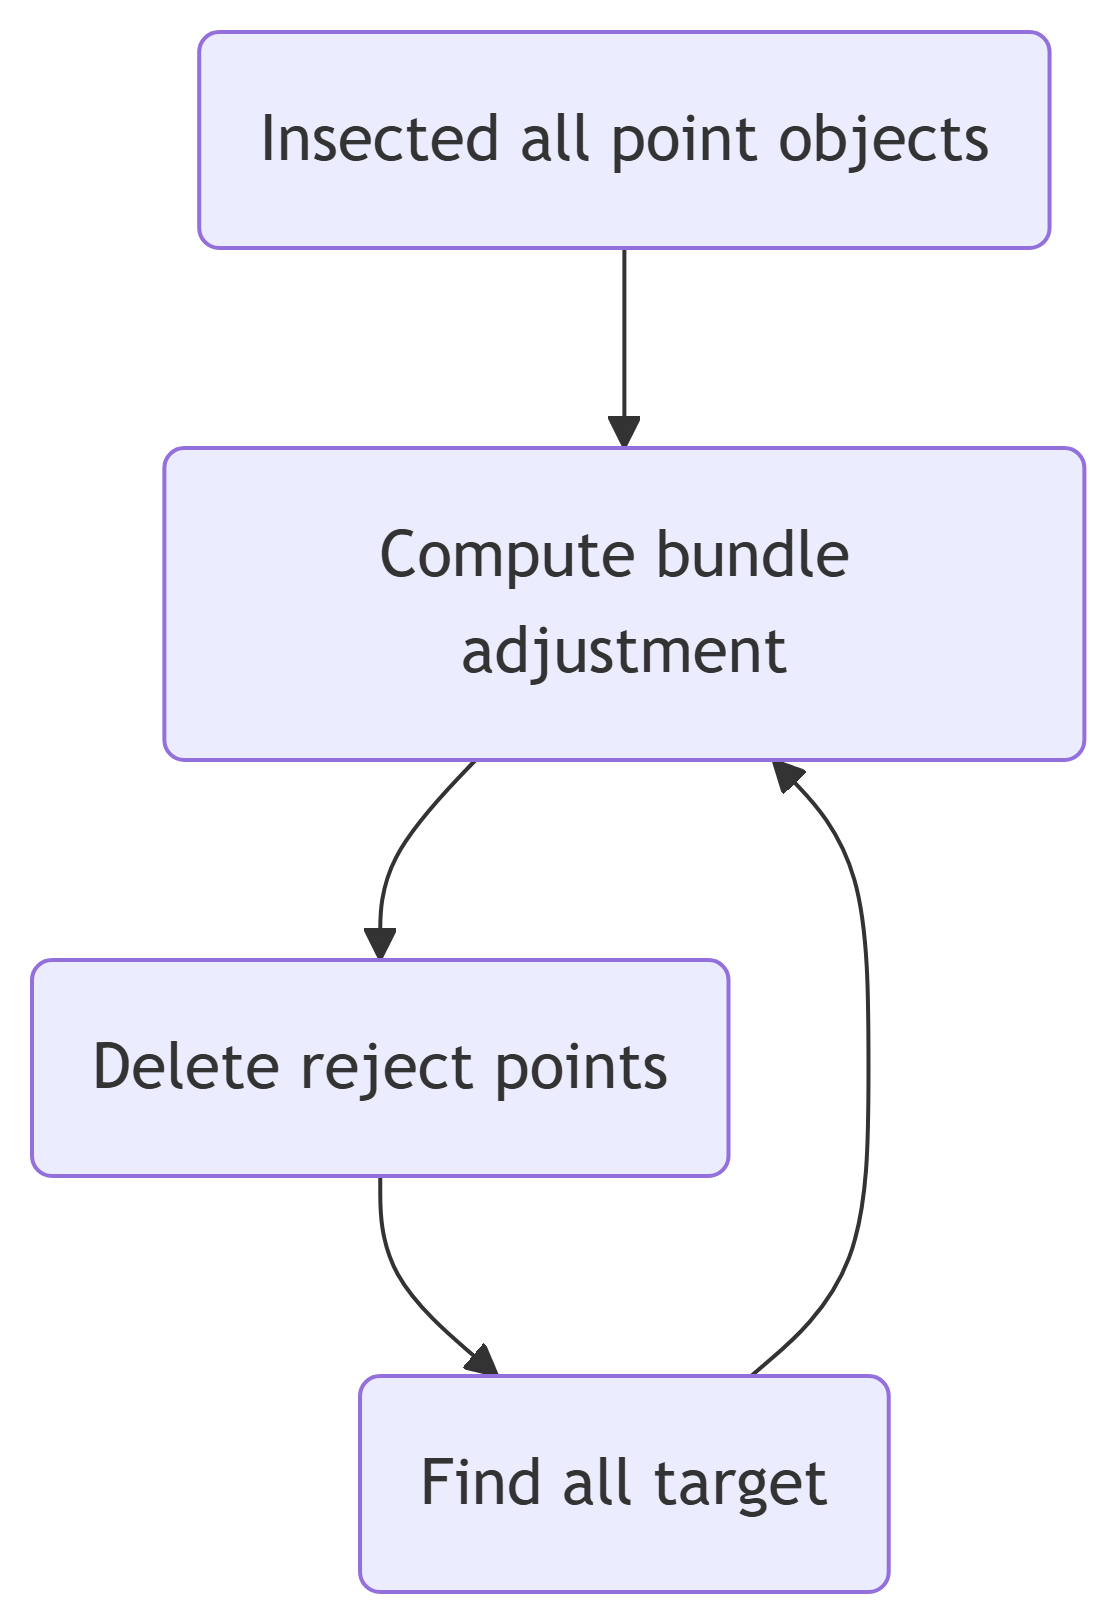
\includegraphics[width=2.91in,height=4.23in]{seagis-cal_files/figure-latex/mermaid-figure-1.png}

Complete a inserção de pontos (objetos) em todas as imagens, depois:
\emph{Adjustment: Compute bundle ajustment} \textgreater{} \emph{Delete
reject points} \textgreater{} \emph{Find target} \textgreater{}
\emph{Compute bundle ajustment\textgreater{} Delete reject points}
\textgreater{} \emph{Compute bundle ajustment} (Final)

\chapter{Manual CAL (pt/br)}\label{manual-cal-ptbr}

\section{\texorpdfstring{\emph{Quick
Guide}}{Quick Guide}}\label{quick-guide}

\begin{quote}
Guia Rápido
\end{quote}

Utilize este guia para percorrer, passo a passo, o processo de
calibração de um sistema de câmeras estéreo. Após capturar e transferir
as imagens de um cubo de calibração, siga as etapas descritas a seguir.

Este guia pressupõe que você já possui arquivos de câmera
(\textbf{.CamCAL}) para iniciar a calibração. Caso isso não seja
verdade, consulte a página de download do software
(\href{https://www.seagis.com.au/download.php}{aqui}) para encontrar
arquivos de câmera comumente utilizados, entre em contato conosco para
obter assistência ou consulte a seção Section~\ref{sec-cameras} para
criar os arquivos necessários.

\begin{tcolorbox}[enhanced jigsaw, opacityback=0, colback=white, colframe=quarto-callout-caution-color-frame, left=2mm, leftrule=.75mm, toprule=.15mm, rightrule=.15mm, breakable, arc=.35mm, bottomrule=.15mm]
\begin{minipage}[t]{5.5mm}
\textcolor{quarto-callout-caution-color}{\faFire}
\end{minipage}%
\begin{minipage}[t]{\textwidth - 5.5mm}

É importante iniciar com arquivos de câmera que você saiba que estão
corretos.

\end{minipage}%
\end{tcolorbox}

\subsection{\texorpdfstring{\emph{Organize the
data}}{Organize the data}}\label{organize-the-data}

\begin{quote}
\emph{Organize os dados}
\end{quote}

\begin{enumerate}
\def\labelenumi{\arabic{enumi}.}
\item
  Usando o \textbf{Explorador de Arquivos do Windows}, crie um novo
  diretório (pasta) para o projeto.
\item
  Copie todos os arquivos de imagem associados à calibração para o novo
  diretório (nova pasta). Normalmente, serão dois arquivos de vídeo: um
  da câmera esquerda e outro da câmera direita.
\item
  Copie para esse diretório o arquivo de pontos do objeto
  (\textbf{.PtsCAL}) do cubo de calibração. \ul{Esse arquivo deve ser
  sempre uma cópia limpa do arquivo original.}
\item
  Copie para esse diretório os arquivos da câmera esquerda e direita
  (\textbf{.CamCAL}). Esses arquivos geralmente são provenientes da
  calibração anterior mais recente.
\end{enumerate}

\subsection{\texorpdfstring{\emph{Create a new
project}}{Create a new project}}\label{create-a-new-project}

\begin{quote}
\emph{Crie um novo projeto}
\end{quote}

\begin{enumerate}
\def\labelenumi{\arabic{enumi}.}
\item
  No CAL, crie um novo projeto usando \textbf{\emph{Project \textbar{}
  New project}}. Se necessário, você será solicitado a salvar quaisquer
  dados não salvos associados ao projeto atual. Insira um nome para o
  arquivo do projeto (por exemplo,
  \textbf{``\textbf{\emph{Calibration}}''}) e salve o arquivo do projeto
  no novo diretório que você acabou de criar para este projeto.
\item
  A criação de um novo projeto inicia um processo de assistente
  (\emph{wizard process}) que solicita a configuração do restante do
  projeto. Basta seguir as instruções, lembrando que todos os arquivos
  estão localizados no mesmo diretório, e que o CAL usará, por padrão, o
  diretório onde o novo arquivo de projeto foi criado.
\item
  Carregue os arquivos da câmera esquerda e direita (\textbf{.CamCAL}),
  conforme solicitado.
\item
  Carregue o arquivo do cubo de calibração (\textbf{.PtsCAL}), conforme
  solicitado.
\item
  Defina o diretório de imagens conforme solicitado. O diretório de
  imagens é automaticamente definido como o mesmo diretório do arquivo
  do projeto; portanto, se todos os arquivos da calibração estiverem em
  um único diretório, basta verificar e clicar em \textbf{OK}.
\item
  Salve o novo arquivo de medições conforme solicitado. Será necessário
  atribuir um nome a esse arquivo (por exemplo,
  \textbf{``\textbf{\emph{Measurements}}''}), e ele será o local onde as
  medições da calibração serão armazenadas.
\item
  Carregue a imagem da câmera esquerda. Normalmente, esse será o arquivo
  de vídeo da câmera esquerda, e ele será automaticamente adicionado à
  configuração da sequência de filmes (Movie sequence) da câmera
  esquerda. Caso existam mais arquivos de vídeo na sequência, eles podem
  ser adicionados nesse momento (ver \textbf{Sequências de filmes}). Em
  seguida, clique em \textbf{OK}.
\item
  Carregue a imagem da câmera direita. Normalmente, esse será o arquivo
  de vídeo da câmera direita, e ele será automaticamente adicionado à
  configuração da sequência de filmes da câmera direita. Caso existam
  mais arquivos de vídeo na sequência, eles podem ser adicionados nesse
  momento (ver \textbf{Sequências de filmes}). Em seguida, clique em
  \textbf{OK}.
\item
  A janela \textbf{\emph{Current project files}} (\emph{Arquivos do
  projeto atual}) será exibida. Todos os campos devem estar preenchidos,
  e todos os itens listados devem estar no mesmo diretório. Clique em
  \textbf{\emph{Close dialog}} (\emph{Fechar diálogo}).
\end{enumerate}

\begin{tcolorbox}[enhanced jigsaw, colframe=quarto-callout-note-color-frame, toprule=.15mm, opacitybacktitle=0.6, opacityback=0, bottomtitle=1mm, colback=white, coltitle=black, left=2mm, toptitle=1mm, titlerule=0mm, leftrule=.75mm, title=\textcolor{quarto-callout-note-color}{\faInfo}\hspace{0.5em}{Note}, rightrule=.15mm, arc=.35mm, breakable, bottomrule=.15mm, colbacktitle=quarto-callout-note-color!10!white]

Se houver dificuldades para chegar a esse ponto, consulte
\textbf{\emph{Creating new projects and data organization}}(), que
fornece mais detalhes ou mostra como configurar o projeto manualmente.

\end{tcolorbox}

\subsection{Medições}\label{mediuxe7uxf5es}

Ao realizar uma calibração de câmeras estéreo, é importante que as
imagens utilizadas na calibração sejam pares estéreo. Se as imagens
usadas na calibração não forem pares estéreo, a segunda etapa da
calibração --- que determina a orientação relativa (configuração
estéreo) das câmeras --- irá falhar.

Ao trabalhar com imagens estáticas, carregue um par estéreo e utilize a
função \emph{Lock}. No caso de arquivos de vídeo, utilize o reprodutor
de vídeo e/ou o avanço quadro a quadro para sincronizar os vídeos
esquerdo e direito, e então utilize a função \emph{Lock} nos vídeos
(veja: a função \emph{Lock}, avanço em vídeos e imagens estáticas, e o
reprodutor de vídeo).

Repita esse procedimento para cada uma das imagens de calibração. Em
geral, devem ser utilizadas 20 imagens para cada câmera (veja o Apêndice
A --- Orientações do cubo de calibração).

A aba \textbf{Images measured} na janela principal do CAL indicará
quantas imagens foram medidas (ao final, esse número deve ser 40: 20
imagens da câmera esquerda e 20 da câmera direita).

\subsection{Ajuste}\label{ajuste}

\begin{enumerate}
\def\labelenumi{\arabic{enumi}.}
\item
  Após concluir todas as medições de imagem, calcule o ajuste de feixe
  usando Ajuste \textbar{} Calcular ajuste de feixe.
\item
  Se você receber uma mensagem de aviso sobre medições de distância
  excluídas ou baixa precisão relativa, ignore-a por enquanto. Se o
  ajuste falhar, consulte os motivos pelos quais um ajuste de feixe pode
  falhar. Se ainda estiver com dificuldades para obter resultados que
  não convergem, tente uma solução apenas com a face frontal, descrita
  em Ajustes com falha em um cubo de calibração SeaGIS.
\item
  Quando o ajuste for bem-sucedido, siga os passos abaixo para produzir
  um conjunto ``limpo'' de medições de imagem, sem rejeições:

  \begin{enumerate}
  \def\labelenumii{\arabic{enumii}.}
  \item
    i. Aceite os resultados do ajuste (usando o botão Aceitar
    resultados).
  \item
    ii. Exclua as medições rejeitadas usando Medição \textbar{} Excluir
    medições de ponto rejeitadas.
  \item
    iii. Procure por alvos ausentes usando Medição \textbar{} Encontrar
    alvos em todas as imagens.
  \item
    iv. Calcule outro ajuste de feixe (Ajuste \textbar{} Calcular ajuste
    de feixe) e aceite os resultados.
  \item
    v. Exclua as medições rejeitadas usando Medição \textbar{} Excluir
    medições de ponto rejeitadas.
  \item
    vi. Calcule um ajuste de feixe final (Ajuste \textbar{} Calcular
    ajuste de feixe). Neste ponto, você deverá ter um ajuste de feixe
    correto. Verifique o seguinte no resumo de Ajuste (uma mensagem de
    aviso alertará sobre possíveis problemas de medição de distância e
    precisão relativa). Você deverá ter \textbf{zero} \emph{Eligible
    image measurements} excluídas e \textbf{zero} \emph{Eligible
    distance measurements} excluídas. Medições de distância excluídas
    podem ser causadas por um cubo montado incorretamente, cubo
    danificado ou medição de locais de pontos de ressecção incorretos --
    este problema deve ser corrigido. Verifique se o valor de precisão
    relativa está de acordo com o esperado para o seu sistema de câmera
    e método de calibração. O CAL possui alguns avisos integrados com
    base em cenários típicos de calibração: geralmente melhor que
    \textbf{1:10.000} para uma calibração estéreo de um sistema de
    câmera de alta definição usando o hardware de calibração SeaGIS.
    Valores mais baixos podem ser causados \hspace{0pt}\hspace{0pt}por
    baixa visibilidade, imagens desfocadas, iluminação inadequada (baixo
    contraste do alvo), número insuficiente de pontos medidos ou cubo
    muito distante das câmeras. Clique em Aceitar resultados.
  \end{enumerate}
\end{enumerate}

\textbf{Observe que o ajuste do feixe precisa ter qualidade aceitável
antes de prosseguir.}

\subsection{Geração de arquivos de câmera
estéreo}\label{gerauxe7uxe3o-de-arquivos-de-cuxe2mera-estuxe9reo}

Note, todas as operações de menu mencionadas nesta seção estão em
\emph{Measurement} \textbar{} \emph{Stereo constraints}.

\begin{enumerate}
\def\labelenumi{\arabic{enumi}.}
\item
  Configure as restrições estéreo usando \emph{Configure stereo
  constraints} . Nesta caixa de diálogo, geralmente basta garantir que a
  câmera esquerda e a câmera direita estejam selecionadas corretamente
  e, em seguida, clicar no botão \emph{Automatic} para gerar os pares
  esquerda/direita. Você receberá uma mensagem de erro se houver um
  número diferente de imagens esquerda e direita medidas, pois o
  software não consegue criar pares estéreo -- você precisará encontrar
  e corrigir a imagem esquerda/direita que não possui uma imagem
  direita/esquerda correspondente (consulte Configurando restrições).
\item
  Estime as restrições usando \emph{Estimating constraints} (consulte
  Estimando restrições). Um aviso será exibido se mais de quatro pares
  estéreo forem excluídos (consulte os comentários na próxima etapa).
\item
  Verifique a orientação relativa usando \emph{View stereo constraints}.
  Verifique se os resíduos de restrição são aceitáveis
  \hspace{0pt}\hspace{0pt}e se não houve muitas restrições que foram
  excluídas do cálculo (coluna \emph{Exclusions}). \textbf{Se mais de
  quatro restrições forem rejeitadas, verifique novamente a
  sincronização estéreo.} Para mais detalhes, consulte Visualizando as
  restrições.
\item
  Gere os arquivos da câmera estéreo usando Exportar arquivos da câmera
  estéreo (consulte Exportando arquivos da câmera estéreo).
\end{enumerate}

\subsection{Salvando resultados}\label{salvando-resultados}

A maneira mais simples de salvar o projeto e todos os dados associados é
fechar o CAL. O programa solicitará que você salve todos os dados não
salvos.

\subsection{Carregando calibrações
anteriores}\label{carregando-calibrauxe7uxf5es-anteriores}

Calibrações anteriores podem ser carregadas clicando duas vezes em um
arquivo de projeto CAL (.PrjCAL) no Explorador de Arquivos do Windows ou
usando o menu CAL \textgreater{} Projeto \textbar{} Ler do arquivo.

Se arquivos (como arquivos de câmera, arquivo de pontos do objeto ou
arquivo de medição) originalmente associados ao projeto tiverem sido
movidos para uma unidade e/ou pasta diferente, o projeto será corrompido
e você precisará recriá-lo manualmente, localizando e carregando os
arquivos necessários. Consulte Recriando um projeto de calibração a
partir de dados existentes.

\section{\texorpdfstring{\emph{General}}{General}}\label{general}

\section{\texorpdfstring{\emph{Installation
details}}{Installation details}}\label{installation-details}

\section{\texorpdfstring{\emph{Project
files}}{Project files}}\label{project-files}

Reading and writing to file

\section{\texorpdfstring{\emph{Cameras}}{Cameras}}\label{sec-cameras}

\begin{quote}
\emph{Câmeras}
\end{quote}

O acesso às informações da câmera e às operações específicas da câmera é
feito por meio do menu \textbf{\emph{Camera}}.

As informações da câmera são armazenadas em um arquivo (um arquivo
separado para cada câmera). Os nomes dos arquivos de câmera atuais são
armazenados no arquivo do projeto e são carregados automaticamente
quando o CAL é iniciado. Observe que esses arquivos de câmera possuem a
extensão \textbf{.CamCAL}. Esses arquivos são diferentes dos arquivos de
câmera estéreo (com extensão \textbf{.Cam}), que o CAL exporta para uso
em softwares de medição estéreo, como o \textbf{EventMeasure} ou o
\textbf{StereoLib}.

\subsection{\texorpdfstring{\emph{Reading and writing to
file}}{Reading and writing to file}}\label{reading-and-writing-to-file}

\begin{quote}
\emph{Leitura e gravação em arquivo}
\end{quote}

As informações da câmera podem ser gravadas em um arquivo ou lidas a
partir de um arquivo. Para ler ou gravar um arquivo de câmera, utilize o
comando de menu \textbf{\emph{Camera \textbar{} Left \textbar{} Read
from file}} ou \textbf{\emph{Camera \textbar{} Left \textbar{} Write to
file}}. Comandos idênticos estão disponíveis para a câmera direita.

Se uma nova câmera for lida a partir de um arquivo ou salva em um
arquivo com um nome diferente, essa alteração será atualizada no arquivo
de projeto atual.

\subsection{\texorpdfstring{\emph{Editing camera
parameters}}{Editing camera parameters}}\label{sec-editing-camera-parameters}

\begin{quote}
\emph{Edição de parâmetros da câmera}
\end{quote}

Para visualizar ou editar os parâmetros de uma câmera, utilize o comando
de menu \textbf{Camera \textbar{} Left \textbar{} Edit parameters} (ou
\textbf{Camera \textbar{} Right \textbar{} Edit parameters} para a
câmera direita). Será exibida uma janela com os seguintes itens:

\begin{longtable}[]{@{}ll@{}}
\toprule\noalign{}
\endhead
\bottomrule\noalign{}
\endlastfoot
& \\
& \\
& \\
& \\
& \\
& \\
& \\
& \\
& \\
& \\
& \\
& \\
& \\
& \\
& \\
\end{longtable}

Itens com um visto verde ao lado podem ser editados dando um duplo
clique no item e digitando um novo valor. Os itens na coluna
\textbf{Units} indicam as unidades do parâmetro. Os valores na coluna
\textbf{Precision} podem ser \textbf{``Fixed parameter''} (parâmetro
fixo) ou um valor numérico. A ausência de valor indica que o parâmetro
da câmera ainda não foi estimado por um ajuste de feixe; já um valor
numérico indica que o parâmetro foi estimado pelo ajuste de feixe, e
esse valor corresponde à precisão do parâmetro.

Os parâmetros \textbf{X Pixel size} e \textbf{Y Pixel size} são
propriedades da câmera e, em geral, podem ser encontrados no site do
fabricante ou em uma ficha técnica ou folha de especificações da câmera.
Frequentemente, o tamanho do pixel precisa ser derivado a partir do
tamanho do sensor da câmera e do formato da imagem. Normalmente, o
fabricante informa esses valores em unidades de micrômetros.
Certifique-se de converter os valores para milímetros (mm) ao inseri-los
como parâmetros da câmera.

Para calibrações de câmera subaquáticas utilizando uma porta plana do
invólucro da câmera, o valor da distância focal em água será
aproximadamente \textbf{4/3} do valor no ar (por exemplo, uma lente com
distância focal de 4,8 mm no ar terá aproximadamente 6,4 mm na água).
Certifique-se de considerar o efeito de quaisquer adaptadores de lente
grande-angular.

Quando uma nova câmera estiver sendo calibrada (isto é, não existe um
arquivo \textbf{.CamCAL} prévio), será necessário especificar:
\textbf{Image rows}, \textbf{Image columns}, \textbf{X Pixel size},
\textbf{Y Pixel size}, e estimar a \textbf{Focal length}. Todos os
demais parâmetros da câmera podem ser inicialmente estimados como zero,
tendo seus valores determinados durante o processo de calibração.

\subsection{\texorpdfstring{\emph{Fixing camera
parameters}}{Fixing camera parameters}}\label{fixing-camera-parameters}

\section{\texorpdfstring{\emph{Pictures}}{Pictures}}\label{pictures}

\section{\texorpdfstring{\emph{Images and
orientations}}{Images and orientations}}\label{images-and-orientations}

\section{\texorpdfstring{\emph{Object points and
distances}}{Object points and distances}}\label{object-points-and-distances}

\section{Medições}\label{mediuxe7uxf5es-1}

\begin{quote}
\emph{Measurement}
\end{quote}

Esta seção aborda o processo de realização de medições de pontos, bem
como descreve o uso dos itens do menu \emph{Measurement}.

\subsection{Pontos de Medida}\label{sec-pontos-medida}

\emph{Point measurement}

\subsection{Salvando e lendo as
medidas}\label{salvando-e-lendo-as-medidas}

\emph{Saving and reading measurements}

\subsection{Convertendo vídeos para
JPEG}\label{convertendo-vuxeddeos-para-jpeg}

\begin{quote}
\emph{Convert movie to JPEG}
\end{quote}

\subsection{Frames deslocados}\label{frames-deslocados}

\emph{Offset frames}

\subsection{Visualizar dados de
orientação}\label{visualizar-dados-de-orientauxe7uxe3o}

\emph{View orientation data}

\subsection{Visualizar/ Excluir medições de
imagem}\label{visualizar-excluir-mediuxe7uxf5es-de-imagem}

\emph{View/ delete image measurement}

\subsection{Resumo das medições de
imagem}\label{resumo-das-mediuxe7uxf5es-de-imagem}

\emph{Image measurement summary}

\subsection{Excluir medições da face
posterior}\label{excluir-mediuxe7uxf5es-da-face-posterior}

\begin{quote}
\emph{Delete back face measurement}
\end{quote}

Ao utilizar um cubo de calibração padrão da SeaGIS, é possível usar
\textbf{\emph{Measurement}} \textbf{\textbar{} \emph{Delete back face
measurement}} para remover todas as medições de imagem associadas a
pontos na face posterior do cubo. Essa função é uma ferramenta útil para
lidar com ajustes de feixe (bundle adjustments) que não convergem; ver
Section~\ref{sec-falha-ajustes}.

\subsection{Cálculo do centróide}\label{cuxe1lculo-do-centruxf3ide}

\emph{Centroiding}

\subsection{Restrições
Estereoscópicas}\label{restriuxe7uxf5es-estereoscuxf3picas}

\emph{Stereo constraints}

Esta seção aborda as opções de menu disponíveis em \emph{Measurement
\textbar{} Stereo constraints}. Essas operações são utilizadas para
configurar \textbf{restrições estereoscópicas} e calcular a
\textbf{orientação relativa} de um par de câmeras estereoscópicas (a
orientação relativa descreve a posição e a orientação de uma câmera em
relação à outra e é necessária para realizar medições com um sistema de
câmeras estereoscópicas). Essas opções são fornecidas principalmente
para gerar arquivos de câmera estereoscópica (extensão \textbf{.cam})
para uso com \emph{PhotoMeasure}, \emph{EventMeasure} e
\emph{StereoLib}.

Em calibrações de câmeras estereoscópicas, a câmera 1 refere-se à câmera
esquerda e a câmera 2 refere-se à câmera direita. O CAL mantém um
sistema de numeração, em vez de utilizar os termos ``Esquerda'' e
``Direita'', para facilitar calibrações genéricas em sistemas com mais
de duas câmeras.

\subsubsection{\texorpdfstring{\textbf{Configuração das
restrições}}{Configuração das restrições}}\label{configurauxe7uxe3o-das-restriuxe7uxf5es}

\emph{Configure constraints}

Use o comando de menu \emph{Configure stereo constraints} para definir
as restrições. Uma janela será exibida. O principal objetivo dessa
janela é permitir a definição de pares estereoscópicos de imagens
esquerda e direita, a partir dos quais a orientação relativa das câmeras
pode ser determinada.

Selecione a câmera esquerda (\emph{Left camera}) e a câmera direita
(\emph{Right camera}) apropriadas usando as caixas de seleção. Na
maioria dos casos, o restante da configuração pode ser realizado
utilizando o botão \emph{Automatic}. Ao clicar em \emph{Automatic}, a
lista de pareamentos será preenchida com combinações de nome do arquivo
da esquerda (nº do frame, nº da câmera) e nome do arquivo da direita (nº
do frame, nº da câmera). Verifique se os pareamentos representam pares
estereoscópicos válidos; caso contrário, será necessário editar a lista
manualmente. Observe que, em calibrações estereoscópicas padrão, a
câmera 1 corresponde à câmera esquerda e a câmera 2 à câmera direita.

Para excluir um pareamento, selecione-o e clique no botão \emph{Delete}.
Para adicionar um pareamento manualmente, selecione um \textbf{Filename}
da câmera esquerda (nº do frame, nº da câmera) e um \textbf{Filename} da
câmera direita (nº do frame, nº da câmera) e clique em \textbf{Add}. Se
algum dos dados recém-adicionados já estiver presente na lista atual de
pareamentos, ele será automaticamente removido e substituído pelo novo
pareamento estereoscópico.

Clique em \textbf{OK} para aceitar a nova configuração ou em
\textbf{Cancel} para ignorar as alterações.

\subsubsection{\texorpdfstring{\textbf{Estimar
restrições}}{Estimar restrições}}\label{sec-estimate.constraint}

\emph{Estimate constraints}

Depois que as restrições estiverem configuradas, a \textbf{orientação
relativa} pode ser estimada. Utilize o comando de menu \emph{Estimate
constraints}. Uma janela será exibida mostrando a orientação relativa
calculada. Os detalhes dessa janela são explicados na seção
\textbf{Viewing the relative orientation}.

Se \textbf{mais de quatro} pares estereoscópicos apresentarem exclusões
associadas, será exibida uma mensagem de aviso. A presença de mais de
quatro pares estereoscópicos com exclusões indica possíveis problemas de
\textbf{sincronização estereoscópica} ou, alternativamente, problemas no
\textbf{ajuste de feixe} (ver \textbf{\emph{Viewing the constraints}}
\{Section~\ref{sec-view.constraint}\} abaixo).

\subsubsection{\texorpdfstring{\textbf{Visualização das
restrições}}{Visualização das restrições}}\label{sec-view.constraint}

\textbf{\emph{Viewing the constraints}}

Depois que as restrições estereoscópicas forem configuradas (ver
\textbf{Configuring constraints}) e estimadas (ver \textbf{Estimating
constraints}, ou estimadas durante um ajuste de feixe), a qualidade da
estimativa pode ser avaliada usando o comando de menu \emph{View stereo
constraints}. Esse comando abre uma janela que exibe cada pareamento
estereoscópico em uma linha, iniciando com o \emph{Filename} da câmera
esquerda e da câmera direita (número do frame, número da câmera).

As colunas seguintes apresentam os \textbf{resíduos} para \emph{Base},
\emph{Delta omega}, \emph{Left phi}, \emph{Left kappa}, \emph{Right phi}
e \textbf{\emph{Right kappa}}. Os resíduos correspondem à diferença
entre a orientação relativa de cada par estereoscópico esquerda/direita
individual e a \textbf{orientação relativa média} calculada a partir de
todos os pares estereoscópicos.

A coluna final lista quaisquer componentes que tenham sido
automaticamente excluídos do cálculo da orientação relativa com base em
seus resíduos (ver \emph{Stereo constraints} para a definição dos
limiares dessas exclusões e para saber quando esses limiares podem
precisar ser ajustados). A magnitude dos resíduos das restrições
estereoscópicas depende, em grande parte, da qualidade da sincronização
das câmeras estereoscópicas. Se uma das restrições apresentar muitos
componentes excluídos, deve-se suspeitar que a sincronização
estereoscópica desse pareamento esquerda/direita esteja incorreta. Isso
frequentemente ocorre devido a movimento excessivo do sistema de câmeras
e/ou da estrutura de calibração, em combinação com um pequeno erro de
sincronização --- possivelmente inferior a um frame --- ou ainda devido
a um erro na seleção do par estereoscópico durante a configuração das
restrições (ver \textbf{Configuring constraints}).

Se muitos dos pares estereoscópicos estiverem sendo excluídos e a
sincronização e a configuração dos pares estiverem corretas, pode ser
necessário \textbf{aumentar os limiares de exclusão}. Para isso, aumente
os valores de \emph{Critical value for base rejection} e/ou
\emph{Critical value for orientation rejection} em \textbf{Stereo
constraints}, e então reestime as restrições conforme descrito em
\textbf{Estimating constraints}. Sempre investigue a sincronização das
imagens estereoscópicas e o pareamento das imagens como a principal
causa das rejeições antes de ajustar esses limiares.

\begin{tcolorbox}[enhanced jigsaw, colframe=quarto-callout-note-color-frame, toprule=.15mm, opacitybacktitle=0.6, opacityback=0, bottomtitle=1mm, colback=white, coltitle=black, left=2mm, toptitle=1mm, titlerule=0mm, leftrule=.75mm, title=\textcolor{quarto-callout-note-color}{\faInfo}\hspace{0.5em}{Note}, rightrule=.15mm, arc=.35mm, breakable, bottomrule=.15mm, colbacktitle=quarto-callout-note-color!10!white]

É impossível obter uma sincronização consistentemente perfeita em
sistemas de câmeras de vídeo estereoscópicas que dependem de
sincronização visual. Nesses sistemas, o erro de sincronização pode
chegar, no pior caso, a meio frame. Esse erro de sincronização, em
combinação com o movimento do sistema de câmeras e/ou da estrutura de
calibração, inevitavelmente resultará em exclusões nas restrições
estereoscópicas. Em função desse erro de sincronização, é aceitável que
até quatro pares estereoscópicos apresentem exclusões.

\end{tcolorbox}

\subsubsection{\texorpdfstring{\textbf{Visualização da orientação
relativa}}{Visualização da orientação relativa}}\label{vis.rel.orient}

\emph{View relative orientation}

Utilize o comando de menu \emph{View relative orientation} para
visualizar os parâmetros atuais da orientação relativa. Uma janela será
exibida. Nessa janela, a origem dos parâmetros(\emph{Parameter source})
será indicada como \emph{Bundle adjustment} se os parâmetros tiverem
sido estimados no ajuste de feixe (ver \textbf{\emph{Stereo
constraints}}); caso contrário, será exibido \emph{Camera positions and
orientations}, o que significa que a orientação relativa foi derivada
das posições e orientações atuais das câmeras. O número de restrições
será igual ao número de restrições configuradas em
\textbf{\emph{Configuring constraints}}.

A separação da base, \emph{Base separation} (X), representa a separação
física entre as câmeras. Em configurações estereoscópicas típicas,
\emph{Delta omega}, \emph{Left kappa} e \emph{Right kappa} tendem a ser
\textbf{próximos de zero}, enquanto \emph{Left phi} e \emph{Right phi}
representam o grau de convergência interna de cada câmera (embora esses
valores também fiquem próximos de zero se as câmeras não convergirem).
Cada parâmetro possui uma precisão associada ao seu cálculo.

\subsubsection{\texorpdfstring{\textbf{Exportando os arquivos de câmera
estereoscópica}}{Exportando os arquivos de câmera estereoscópica}}\label{sec-exp.stereo.files}

\emph{Exporting stereo camera files}

Para exportar arquivos de câmera estereoscópica, as restrições
estereoscópicas devem estar configuradas (ver \textbf{\emph{Configuring
constraints}}), estimadas (ver \textbf{\emph{Estimating constraints}},
ou estimadas durante um ajuste de feixe) e os resultados verificados
(ver \textbf{\emph{Viewing the constraints}}). Em seguida, os arquivos
de câmera estereoscópica podem ser criados usando o comando de menu
\emph{Export stereo camera files}.

Se as restrições não tiverem sido configuradas ou estimadas, será
exibida uma mensagem de erro. Inicialmente, os parâmetros da câmera
esquerda serão mostrados em uma janela. Clique no botão \emph{Close} da
caixa de diálogo e uma mensagem solicitará que você salve os parâmetros
da câmera esquerda. Clique em \emph{Yes}, e uma janela padrão do Windows
será exibida, permitindo selecionar o nome do arquivo de câmera
estereoscópica para a câmera esquerda.

Após o salvamento do arquivo da câmera esquerda, uma nova janela será
exibida com os parâmetros da câmera direita. Clique no botão
\textbf{Close} da caixa de diálogo, e uma mensagem solicitará que você
salve os parâmetros da câmera direita. Clique em \textbf{Yes} para abrir
a janela do Windows, na qual será possível selecionar o nome do arquivo
da câmera direita.

\subsection{Ressecção de todas as
imagens}\label{ressecuxe7uxe3o-de-todas-as-imagens}

\emph{Resect all images}

O comando de menu \emph{Measurement \textbar{} Resect all images} na
janela principal do CAL calcula uma ressecção em cada uma das imagens
associadas ao projeto atual. Ao término do processo de ressecção, uma
janela com um relatório resumido é exibida. A janela lista todas as
imagens envolvidas na operação de ressecção, se a ressecção foi
bem-sucedida e o erro RMS associado à ressecção. Consulte os botões
Ressecção e Encontrar alvos automaticamente para obter mais informações
sobre ressecções. Observe que pelo menos quatro pontos de ressecção
devem ser medidos em uma imagem antes que ela possa ser ressecada.

Essa opção geralmente não é usada, pois as imagens normalmente são
ressecadas individualmente à medida que são medidas.

\subsection{Encontrar alvos em todas as
imagens}\label{encontrar-alvos-em-todas-as-imagens}

O comando de menu Medição \textbar{} Encontrar alvos em todas as imagens
executa um processo automático no qual todas as imagens do projeto atual
são carregadas e uma tentativa é feita para medir quaisquer pontos de
objeto não medidos em cada imagem. Enquanto esse processo estiver em
execução, uma janela de progresso será exibida. O processo pode ser
cancelado a qualquer momento clicando no botão Cancelar na janela de
progresso.

Essa opção geralmente é usada após um ajuste de feixe bem-sucedido. Após
um ajuste de feixe, os parâmetros da câmera apresentam melhor qualidade
e é provável que mais pontos de objeto possam ser medidos
automaticamente. O procedimento geral consiste em excluir as medições
excluídas pelo ajuste de feixe e, em seguida, executar esse processo
para medir automaticamente quaisquer pontos de objeto não medidos. O
ajuste de feixe pode então ser recalculado (consulte mais detalhes em
Calculando o ajuste).

Observe que esse processo tentará encontrar (em cada imagem) apenas os
pontos de objeto que atualmente não possuem medição. Se um ponto já
estiver medido, a medição atual do ponto será mantida sem alterações.

\subsection{Intersecção de todos os
pontos}\label{intersecuxe7uxe3o-de-todos-os-pontos}

O comando de menu Medição \textbar{} Intersecção de todos os pontos
utiliza as posições e orientações atuais da câmera para todas as imagens
e intersecta todas as medições da imagem para calcular as coordenadas do
objeto. Essa funcionalidade é usada para estimar as coordenadas do
espaço do objeto para pontos recém-medidos.

Ao realizar ajustes de feixe com cubos de calibração, essa opção não é
utilizada.

\subsection{Excluir medições de pontos
rejeitadas}\label{excluir-mediuxe7uxf5es-de-pontos-rejeitadas}

O comando de menu Medição \textbar{} Excluir medições de pontos
rejeitadas excluirá todas as medições de pontos que foram marcadas como
rejeitadas (as medições de pontos podem ser rejeitadas por ressecções,
intersecções ou ajuste de feixe; consulte Cores de pontos, Valores para
rejeição de medição). Essa função é normalmente usada após um ajuste de
feixe para excluir todas as medições de pontos rejeitadas.

Quarto enables you to weave together content and executable code into a
finished document. To learn more about Quarto see
\url{https://quarto.org}.

\section{\texorpdfstring{\textbf{Ajuste}}{Ajuste}}\label{ajuste-1}

\begin{quote}
\emph{Adjustment}
\end{quote}

Esta seção trata dos comandos de menu disponíveis no menu
\textbf{\emph{Adjustment}}. Esses comandos são usados para configurar e
executar um ajuste do fardo das imagens (\emph{bundle adjustment}).
Antes de calcular um ajuste de fardo, é necessário realizar a
\textbf{resseção} de todas as imagens, ver
Section~\ref{sec-pontos-medida}, e medir a maioria dos alvos na maioria
das imagens (preferencialmente, todos os alvos visíveis em todas as
imagens).

\subsection{Critérios de
convergência}\label{crituxe9rios-de-converguxeancia}

\begin{quote}
\emph{Convergence criteria}
\end{quote}

Durante o ajuste do fardo, os parâmetros (coordenadas dos pontos do
objeto, posições e orientações da câmera e parâmetros de calibração da
câmera) convergem para um valor final. O grau de convergência pode ser
ajustado com precisão, se necessário. Consulte também
Section~\ref{sec-cal-ajuste}.

\subsubsection{\texorpdfstring{\emph{Object
points}}{Object points}}\label{object-points}

\begin{quote}
\emph{Pontos do objeto}
\end{quote}

Para ajustar os \emph{critérios de convergência} dos pontos do objeto,
use o comando de menu \textbf{\emph{Adjustment \textbar{} Object point
convergence criteria}}. Uma janela será exibida, permitindo o ajuste dos
critérios de convergência. Esse valor geralmente pode ser definido como
1/1000 das unidades do espaço do objeto, por exemplo, 1 mícron se as
unidades do espaço do objeto forem milímetros.\footnote{Portanto, 10
  mícrons se a unidade de espaço do objeto for em centímetros (1 cm =
  10000 mícrons).}

\subsubsection{\texorpdfstring{\emph{Camera positions and
orientations}}{Camera positions and orientations}}\label{camera-positions-and-orientations}

\begin{quote}
\emph{Posições e orientações da câmera}
\end{quote}

Para ajustar os \emph{critérios de convergência} da posição e orientação
da câmera, use o comando de menu \textbf{\emph{Adjustment \textbar{}
Camera position and orientation convergence criteria}}. Uma janela será
exibida, permitindo o ajuste dos critérios de convergência. Há dois
valores: um para as orientações da câmera em unidades de segundos de
arco e outro para a posição da câmera. As unidades para a posição da
câmera serão em unidades do espaço do objeto x 1000. Os valores padrão
são 1 segundo de arco para orientação e 1/1000 das unidades do espaço do
objeto para posição (por exemplo, 1 mícron se as unidades do espaço do
objeto forem milímetros).

\subsubsection{\texorpdfstring{\emph{Camera
parameters}}{Camera parameters}}\label{camera-parameters}

\begin{quote}
\emph{Parâmetros da câmera}
\end{quote}

Os \emph{critérios de convergência} para os parâmetros da câmera podem
ser definidos usando o comando de menu \textbf{\emph{Adjustment
\textbar{} Camera convergence criteria}}. Cada um dos parâmetros da
câmera (consulte Section~\ref{sec-editing-camera-parameters}) possui
\ul{seus próprios critérios de convergência}. A tabela a seguir fornece
os valores padrão para os critérios de convergência da câmera.

\subsection{Ajustes de
configuração}\label{ajustes-de-configurauxe7uxe3o}

\begin{quote}
\emph{Adjustment settings}
\end{quote}

As configurações do \emph{bundle adjustment} são controladas por meio do
comando de menu \textbf{\emph{Adjustment \textbar{} Adjustment
settings}}. Uma janela é exibida, permitindo configurar os parâmetros do
ajuste. A seguir, são descritas as configurações e apresentados valores
padrão recomendados.

\subsubsection{Valores para medida de
rejeição}\label{valores-para-medida-de-rejeiuxe7uxe3o}

\emph{Values for measurement rejection}

Esses valores controlam a exclusão automática de medições de
determinados cálculos quando se determina que a medição provavelmente
contém erro.

\begin{itemize}
\item
  \textbf{Nome:} Valor crítico para rejeição na ressecção.\\
  \textbf{Padrão:} 3,00 pixels.\\
  \textbf{Descrição:} Quando um ponto medido é utilizado em um cálculo
  de ressecção e o resíduo resultante é maior que esse valor, ele é
  excluído do cálculo. Quando isso ocorre, a cor do ponto é alterada
  para \textbf{Point colour, residual failed} (veja \emph{Point
  colours}).
\item
  \textbf{Nome:} Valor crítico para rejeição na interseção.\\
  \textbf{Padrão:} 3,00 pixels.\\
  \textbf{Descrição:} Quando um ponto medido é utilizado em um cálculo
  de interseção e o resíduo resultante é maior que esse valor, ele é
  excluído do cálculo. Quando isso ocorre, a cor do ponto é alterada
  para \textbf{Point colour, residual failed} (veja \emph{Point
  colours}).
\item
  \textbf{Nome:} Valor crítico para rejeição no \emph{bundle
  adjustment}.\\
  \textbf{Padrão:} 2,50 pixels.\\
  \textbf{Descrição:} Quando um ponto medido é utilizado no \emph{bundle
  adjustment} e o resíduo resultante é maior que esse valor, ele é
  excluído do ajuste. Quando isso ocorre, a cor do ponto é alterada para
  \textbf{Point colour, residual failed} (veja \emph{Point colours}).
\item
  \textbf{Nome:} Fator de rejeição para distâncias no espaço do
  objeto.\\
  \textbf{Padrão:} 5,00.\\
  \textbf{Descrição:} Esse fator é usado para definir um valor crítico
  (valor crítico = desvio padrão da medição de distância × fator de
  rejeição para distâncias no espaço do objeto) para remover distâncias
  de um \emph{bundle adjustment}. Quando o resíduo de uma distância no
  \emph{bundle adjustment} excede esse valor crítico, ela é excluída do
  ajuste.
\item
  \textbf{Nome:} Fator de rejeição para restrições de coordenadas.\\
  \textbf{Padrão:} 5,00.\\
  \textbf{Descrição:} Esse fator é usado para definir um valor crítico
  (valor crítico = desvio padrão da restrição de coordenadas × fator de
  rejeição para restrições de coordenadas) para remover restrições de
  coordenadas de um \emph{bundle adjustment}. Quando o resíduo de uma
  restrição de coordenadas no \emph{bundle adjustment} excede esse valor
  crítico, ela é excluída do ajuste.
\item
  \textbf{Nome:} \% do valor crítico para cor de ponto de aviso.\\
  \textbf{Padrão:} 80,0\%.\\
  \textbf{Descrição:} Veja \emph{Point colours}. Esse valor pode ser
  configurado na janela de cores dos pontos e é descrito lá.
\end{itemize}

\subsubsection{\texorpdfstring{\textbf{Precisão de medição de
imagem}}{Precisão de medição de imagem}}\label{precisuxe3o-de-mediuxe7uxe3o-de-imagem}

\emph{Image measurement precision}

\begin{itemize}
\item
  \textbf{Nome:} Desvio padrão da medição de imagem.\\
  \textbf{Padrão:} 0,10 pixels.\\
  \textbf{Descrição:} Define o desvio padrão para as medições na imagem.
  Como regra geral, utilize 0,10 pixels para medições feitas com
  \emph{centroiding} e entre 0,50 e 1,00 pixels para medições feitas
  manualmente (apenas com o uso do mouse). Esse valor influencia a
  precisão dos parâmetros estimados no \emph{bundle adjustment} APENAS
  se o parâmetro a seguir estiver definido como \textbf{FALSE}. Definir
  corretamente esse valor é importante para simulações.
\item
  \textbf{Nome:} Reponderar observações de imagem usando sigma zero.\\
  \textbf{Padrão:} True.\\
  \textbf{Descrição:} Quando definido como \textbf{true} e ao executar
  um \emph{bundle adjustment}, o desvio padrão das medições de imagem
  (descrito acima) será automaticamente ajustado para produzir um valor
  de sigma zero igual a 1 (± 0,05). Isso fornece automaticamente a
  ``melhor'' estimativa das precisões dos parâmetros. Esse valor
  normalmente deve ser mantido como \textbf{true}, a menos que você
  esteja realizando uma simulação. Note que apenas os desvios padrão das
  medições de imagem são alterados (o desvio padrão das medições de
  distância ou das restrições de coordenadas não é alterado). A nova
  estimativa do desvio padrão da medição de imagem é exibida no resumo
  dos resultados do ajuste (veja \emph{Computing the adjustment}).
\end{itemize}

\subsubsection{Restrições estéreo}\label{restriuxe7uxf5es-estuxe9reo}

Os parâmetros a seguir são relevantes apenas quando o objetivo do
\emph{bundle adjustment} é estimar os parâmetros de uma configuração de
câmera estéreo.

\begin{itemize}
\item
  \textbf{Nome:} Usar restrição estéreo.\\
  \textbf{Padrão:} False.\\
  \textbf{Descrição:} Quando definido como \textbf{true}, os parâmetros
  de orientação relativa são estimados (ou, mais precisamente,
  restringidos) durante o \emph{bundle adjustment}. Na prática, cada par
  de imagens esquerda/direita é forçado a resultar na mesma orientação
  relativa, dentro dos limites definidos por \textbf{SD for stereo base
  constraint} e \textbf{SD for stereo orientation constraint} (veja
  abaixo).
\item
  \textbf{Nome:} Valor crítico para rejeição da base.\\
  \textbf{Padrão:} 5000,0 micrômetros.\\
  \textbf{Descrição:} Durante o cálculo da orientação relativa (seja
  como parte do \emph{bundle adjustment} ou usando \emph{Estimating
  constraints}), qualquer componente da base que exceda esse valor para
  um par de imagens esquerda/direita será ignorado. As unidades
  utilizadas para esse parâmetro dependem do projeto atual. Esse valor
  pode precisar ser aumentado caso a sincronização estéreo das câmeras
  não seja perfeita (comum em sistemas de vídeo).
\item
  \textbf{Nome:} Valor crítico para rejeição da orientação.\\
  \textbf{Padrão:} 1800 segundos de arco.\\
  \textbf{Descrição:} Durante o cálculo da orientação relativa (seja
  como parte do \emph{bundle adjustment} ou usando \emph{Estimating
  constraints}), qualquer componente de orientação que exceda esse valor
  para um par de imagens esquerda/direita será ignorado. Esse valor pode
  precisar ser aumentado caso a sincronização estéreo das câmeras não
  seja perfeita (comum em sistemas de vídeo).
\item
  \textbf{Nome:} Desvio padrão (SD) para restrição da base estéreo.\\
  \textbf{Padrão:} 100,0 micrômetros.\\
  \textbf{Descrição:} Quando \textbf{Use stereo constraint} (veja acima)
  está definido como \textbf{true}, este é o valor de restrição aplicado
  a todos os pares de imagens esquerda/direita para o componente da base
  da orientação relativa. As unidades desse parâmetro dependem das
  unidades do projeto atual. Essa restrição pode precisar ser relaxada
  caso a sincronização estéreo das câmeras não seja perfeita (comum em
  sistemas de vídeo).
\end{itemize}

\subsection{Cálculo do Ajuste}\label{sec-cal-ajuste}

\begin{quote}
\emph{Computing the adjustment}
\end{quote}

Após todas as imagens serem ressecadas e os alvos medidos em todas elas,
o ajuste de feixe pode ser calculado. Para executar o ajuste de feixe,
use o comando de menu \emph{Adjustment \textbar{} Compute bundle
adjustment} na janela principal do CAL. Uma janela de progresso é
exibida com um botão Cancelar. O ajuste pode ser cancelado a qualquer
momento clicando no botão Cancelar (o processo não será cancelado até
que a iteração atual seja calculada). A janela exibe informações sobre o
progresso do ajuste (o número da iteração) e o sigma zero (que indica a
qualidade do ajuste e idealmente deve estar próximo de 1). O ajuste
primeiro calcula uma solução inicial, seguida por uma série de soluções
de reponderação, onde as medições de baixa qualidade são removidas
automaticamente do ajuste. Finalmente, as precisões e correlações dos
parâmetros são calculadas.

Nesta etapa, haverá um ajuste convergido com sucesso ou um ajuste que
não convergiu. Uma nova janela será exibida. Essa janela contém duas
caixas de listagem: a caixa de listagem superior exibe um resumo do
ajuste em texto, e a caixa de listagem inferior exibe detalhes sobre o
ajuste.

Uma caixa de mensagem pode ser exibida com avisos sobre medições de
distância excluídas e/ou baixa precisão relativa. Os avisos são baseados
em cenários típicos de calibração de câmeras estéreo usando o hardware
de calibração SeaGIS. Nesses casos, o ajuste final do feixe não deve
apresentar medições de distância excluídas, e há expectativas em relação
à precisão relativa. Veja detalhes nos tópicos a seguir. Ignore o aviso
se ele não se aplicar especificamente ao seu uso do CAL.

Considerando o resumo do ajuste, a primeira linha indicará se o ajuste
convergiu com sucesso ou se houve falha. Outras informações fornecidas
serão:

\begin{itemize}
\tightlist
\item
  Indica se as observações da imagem foram reponderadas para obter um
  sigma zero de 1 (consulte Precisão da medição da imagem) e se a
  reponderação foi bem-sucedida. O valor de sigma zero é fornecido,
  assim como a nova estimativa da precisão da medição da imagem.
\end{itemize}

\begin{itemize}
\tightlist
\item
  Indica se algum aspecto do processo de ajuste falhou e, em caso
  afirmativo, fornece uma indicação do que deu errado. Isso pode incluir
  falha na convergência dentro do número máximo de iterações (consulte
  Ajuste) ou falha na resolução das equações normais (isso geralmente
  indica que não foram medidos pontos de objeto suficientes em imagens
  suficientes ou pode ser causado por restrições de pontos de objeto sem
  sentido).
\end{itemize}

\begin{itemize}
\tightlist
\item
  O resíduo médio da imagem (\textbf{geralmente deve ser sempre menor
  que 0,3 pixels}).
\end{itemize}

\begin{itemize}
\tightlist
\item
  O número total de parâmetros do modelo de ajuste, parâmetros restritos
  e redundâncias. \textbf{O número de redundâncias para uma calibração
  de câmera estéreo geralmente será da ordem de 5.000}.
\end{itemize}

\begin{itemize}
\tightlist
\item
  O número de medições de imagem e distância elegíveis e excluídas, e
  restrições de pontos de objeto. As medições excluídas não atenderam
  aos parâmetros definidos em Valores para rejeição de medição. Após um
  ajuste inicial, pode haver muitas medições de imagem elegíveis
  excluídas. Isso é normal. Ao usar o hardware de calibração do SeaGIS
  (um cubo), não deve haver nenhuma medição de distância elegível
  excluída -- isso pode indicar: um cubo montado incorretamente, um cubo
  danificado ou localizações de pontos de ressecção medidas
  incorretamente.
\end{itemize}

\begin{itemize}
\tightlist
\item
  Avisos se houver pontos no espaço do objeto que não possuem
  coordenadas estimadas. Isso ocorrerá se novos pontos do objeto forem
  adicionados sem estimativas de coordenadas (isso nunca deve acontecer
  com projetos de cubo de calibração). Use a interseção para estimar as
  coordenadas (consulte Interseccionar todos os pontos).
\end{itemize}

\begin{itemize}
\tightlist
\item
  Avisos se houver distâncias medidas para pontos do objeto que não
  existem ou para pontos do objeto que não possuem coordenadas
  estimadas.
\end{itemize}

\begin{itemize}
\tightlist
\item
  Avisos se houver posições de câmera não selecionadas (consulte Medição
  de ponto).
\end{itemize}

\begin{itemize}
\tightlist
\item
  Avisos se houver medições de imagem feitas para pontos de objeto que
  não existem ou para pontos de objeto que não possuem uma coordenada
  estimada.
\end{itemize}

\begin{itemize}
\tightlist
\item
  Avisos se houver medições associadas a uma câmera que não faz parte de
  um projeto (pode ocorrer se uma câmera for excluída de um projeto
  existente, mas ainda houver medições associadas à câmera excluída).
\end{itemize}

\begin{itemize}
\tightlist
\item
  Avisos se forem usadas restrições estéreo e as restrições não tiverem
  sido estimadas ou envolverem posições de câmera inválidas ou não
  estimadas (consulte Restrições estéreo).
\end{itemize}

\begin{itemize}
\tightlist
\item
  A precisão relativa (consulte View object point summary). Para a
  calibração estéreo de um sistema de câmera de alta definição usando o
  hardware de calibração do SeaGIS (um cubo), \textbf{esse valor deve
  ser em torno de 1:10.000} ou melhor. A precisão relativa pode ser
  prejudicada por: baixa visibilidade, iluminação inadequada (baixo
  contraste do alvo), imagens desfocadas, número insuficiente de pontos
  medidos ou cubo muito distante das câmeras.
\end{itemize}

Se o ajuste não convergir, os parâmetros que não estão convergindo serão
relatados. A não convergência geralmente está associada a uma geometria
de rede inadequada ou a um número insuficiente de medições em imagens
suficientemente diferentes (isso nunca deve ocorrer com redes de
calibração que envolvem cubos de calibração, como no Apêndice A -
Orientações do cubo de calibração). Para forçar a convergência do
ajuste, os critérios de convergência para os parâmetros que estão
falhando podem ser ajustados para forçar a rede a convergir (consulte
Critérios de convergência) ou o número máximo de iterações para o ajuste
do feixe pode ser aumentado temporariamente (consulte Ajuste).

A caixa de listagem Detalhes fornece informações mais detalhadas sobre
os resultados do ajuste. Todos os itens listados podem ser visualizados
com mais detalhes clicando duas vezes sobre o item. As seguintes
informações são fornecidas:

\begin{itemize}
\tightlist
\item
  Parâmetros da câmera: Para cada câmera, um resumo dos parâmetros da
  câmera. Essas informações são as mesmas exibidas em Edição de
  parâmetros da câmera. Certifique-se de que a distância focal esteja
  correta. Todos os outros parâmetros devem ter uma magnitude pequena --
  parâmetros com grande magnitude indicam um problema.
\end{itemize}

\begin{itemize}
\tightlist
\item
  Resumo dos pontos do objeto. Essas informações são as mesmas exibidas
  em Visualização do resumo dos pontos do objeto. \textbf{Verifique se a
  precisão relativa está correta. O número de pontos não estimados deve
  ser 0. O intervalo entre os desvios padrão máximo e mínimo dos pontos
  deve ser pequeno.} Se o desvio padrão máximo dos pontos for muito
  grande, isso indica que alguns pontos do objeto não foram medidos o
  suficiente para estimar as coordenadas com precisão. Esses pontos
  devem ser identificados e mais medições de imagem devem ser feitas
  nesses pontos.
\end{itemize}

\begin{itemize}
\tightlist
\item
  Coordenadas/precisões dos pontos do objeto. Essas informações são as
  mesmas exibidas em Viewing and manipulating object space points
  (Visualização e manipulação de pontos no espaço do objeto).
  \textbf{Nesta janela, identifique os pontos que apresentam desvios
  padrão maiores que a média (sX, sY, sZ)}. Geralmente, eles terão um
  número menor de medições (Nº de Obs.) em comparação com outros pontos.
  É necessário realizar mais medições de imagem nesses pontos. Verifique
  rapidamente se as coordenadas dos pontos do objeto estão dentro do
  intervalo esperado.
\end{itemize}

\begin{itemize}
\tightlist
\item
  Orientação e posições da câmera (e observações da imagem). Essas
  informações são as mesmas exibidas em Dados de orientação da imagem.
  Nesta janela, examine todas as posições e orientações da câmera e
  certifique-se de que os valores sejam razoáveis
  \hspace{0pt}\hspace{0pt}(observe especialmente as posições da câmera
  que não se encaixam). \textbf{Observe a precisão das posições da
  câmera (sX, sY, sZ) e das orientações (sOmega, sPhi, sKappa), bem como
  o número de medições em cada imagem (Nº de obs.)}. Esses valores devem
  ter magnitude semelhante em todas as imagens. Se uma imagem apresentar
  um desempenho particularmente pior, pode ser porque ela não possui
  medições suficientes dos pontos do objeto ou porque a qualidade da
  imagem pode ser inferior. Você também pode examinar as medições e os
  resíduos de uma imagem específica clicando duas vezes nela, embora o
  Resumo de resíduos da imagem abaixo possa ser mais útil.
\end{itemize}

\begin{itemize}
\tightlist
\item
  Resumo de resíduos da imagem. Estas são as mesmas informações
  descritas em Resumo de medições da imagem. \textbf{Analise os resíduos
  médios da imagem e identifique quaisquer imagens que apresentem uma
  média visivelmente maior do que as demais.} Investigue as medições
  e/ou a qualidade da imagem associadas a essas imagens. Frequentemente,
  uma imagem com uma média alta pode ter pontos de ressecção mal
  identificados ou medições feitas em alvos mal identificados. Nesses
  casos, é prudente excluir todas as medições da imagem com uma média
  alta e medi-la novamente. Uma média alta também pode ser causada por
  baixa qualidade da imagem (geralmente desfoque de movimento).
\end{itemize}

\begin{itemize}
\tightlist
\item
  Todas as medições da imagem. Estas são as mesmas informações exibidas
  em Visualizar/excluir medições da imagem. Classifique os dados nesta
  janela clicando duas vezes na coluna Rejeitadas para trazer todas as
  medições rejeitadas para o topo. Observe se as medições rejeitadas
  tendem a estar associadas a um ou mais pontos do objeto. Nesse caso,
  investigue todas as medições até o(s) ponto(s) específico(s) do
  objeto, pois a medição pode ter sido feita no ponto errado.
\end{itemize}

\begin{itemize}
\tightlist
\item
  Medições de distância. Esta opção só será exibida se houver medições
  de distância. As informações são as mesmas exibidas em Visualizando e
  manipulando distâncias. Verifique se alguma distância está sendo
  excluída (isso não deve acontecer com um cubo de calibração e indica
  que o cubo ou os alvos nele contidos podem ter sido danificados
  fisicamente).
\end{itemize}

\begin{itemize}
\tightlist
\item
  Visualizar correlações. Clicar duas vezes neste item abre outra janela
  que permite visualizar as correlações entre os parâmetros. Insira o
  coeficiente de correlação desejado; quaisquer parâmetros acima do
  coeficiente de correlação especificado serão relatados. Você pode
  optar por incluir ou excluir os parâmetros de posição e orientação
  (orientação externa) da câmera, conforme necessário. Após a
  configuração, clique no botão Fechar caixa de diálogo e uma nova
  janela será exibida mostrando quaisquer parâmetros correlacionados. Se
  a janela estiver vazia, não havia parâmetros acima dos limites
  prescritos.
\end{itemize}

\begin{itemize}
\tightlist
\item
  Restrições estéreo e resíduos. Esses dados só aparecerão se você usar
  restrições estéreo no ajuste de feixe (consulte Restrições estéreo).
  As informações e a interpretação são as mesmas que em Visualizando as
  restrições. Se muitos dos componentes de restrição estéreo estiverem
  sendo excluídos, a ponderação da restrição pode precisar ser relaxada
  (consulte Restrições estéreo).
\end{itemize}

\begin{itemize}
\tightlist
\item
  ~Restrições estéreo -- orientação relativa. Esses dados só aparecerão
  se você usar restrições estéreo no ajuste de feixe (consulte
  Restrições estéreo). As informações e a interpretação são as mesmas
  que em Visualizando a orientação relativa.
\end{itemize}

Se o ajuste for bem-sucedido, o botão Aceitar na parte inferior da
janela será habilitado. Após avaliar os resultados do ajuste e
certificar-se de que o resultado é válido, clique no botão Aceitar para
adotar o resultado do ajuste de feixe. Ao clicar no botão Aceitar, os
parâmetros da câmera, as coordenadas dos pontos do objeto e as posições
e orientações da câmera são atualizados com os resultados calculados no
ajuste de feixe. Se o ajuste falhar ou o resultado não for satisfatório,
clique no botão Cancelar para ignorar os resultados do ajuste.
\textbf{Nunca aceite os resultados de um ajuste de feixe questionável}.

Após concluir um ajuste de feixe bem-sucedido, é recomendável excluir as
medições de imagem que foram excluídas pelo ajuste (consulte Excluir
medições de pontos rejeitadas).

Se houver muitos pontos do objeto que não foram medidos com sucesso
(como geralmente ocorre quando não há informações de calibração
anteriores para uma câmera), esses pontos agora devem ser medidos
automaticamente com sucesso. Assim que o ajuste de feixe for calculado
com sucesso, haverá parâmetros de calibração da câmera melhores,
permitindo que os alvos não medidos sejam medidos automaticamente. O
procedimento para medição automática de todas as imagens do projeto é
descrito em Encontrar alvos em todas as imagens. Após a medição de mais
alvos, o ajuste do feixe pode ser recalculado. Observe que nunca será
possível medir todos os alvos em todas as imagens, pois alguns alvos
inevitavelmente estarão ocluídos.

\subsection{Razões pelas quais um ajuste de feixe pode
falhar}\label{razuxf5es-pelas-quais-um-ajuste-de-feixe-pode-falhar}

Às vezes, o ajuste de feixe pode falhar, e pode ser difícil identificar
exatamente por que isso está acontecendo. A seguir estão algumas razões
e soluções comuns:

\begin{itemize}
\tightlist
\item
  O ajuste pode não convergir devido a uma ou duas medições realmente
  ruins. Se for possível forçar o ajuste a convergir ao menos uma vez,
  essas medições problemáticas serão identificadas e removidas.
\end{itemize}

\emph{Ajuste o máximo de interações usando o} Ajustment \textbar{}
Ajustment \emph{settings e ponha o} Maximum iterations \emph{em 500.}

\begin{itemize}
\tightlist
\item
  Medições insuficientes para pontos suficientes. Às vezes, há uma
  tendência de calcular o ajuste de feixe antes de realizar medições
  suficientes em um número adequado de pontos do objeto e em imagens
  suficientes. Quando isso ocorre, o ajuste de feixe pode falhar
  completamente ou não convergir. Nesse caso, é simplesmente necessário
  realizar mais medições. O ajuste de feixe depende de redundância
  (muitas medições) para detectar e eliminar de forma confiável medições
  errôneas. Se não houver medições suficientes, a detecção correta
  dessas medições incorretas torna-se difícil e pode levar à falha do
  ajuste de feixe.
\end{itemize}

\emph{Não se preocupe em calcular o ajuste de feixe até que toda a
sequência de calibração tenha sido medida (ver} Apêndice A ---
Orientações do cubo de calibração\emph{). Se o processo de centroiding
não estiver encontrando muitos pontos, tente ajustar o brilho e o
contraste da imagem para realçar os alvos} (Brightness and contrast).
\emph{Também pode ser necessário ajustar a configuração de centróide
``Minimum Pixel Intensity Range'', reduzindo esse valor (}Editing and
fine tuning settings\emph{).}

\begin{itemize}
\tightlist
\item
  Um ajuste pode falhar se pontos medidos tiverem sido atribuídos a um
  ID de ponto incorreto. Se um ponto for medido de forma consistente e
  receber um ID incorreto em muitas imagens, isso causará confusão no
  ajuste de feixe (ou seja, o ajuste de feixe não conseguirá identificar
  com precisão que o ponto incorreto foi medido). Isso pode se tornar um
  problema sério se os pontos iniciais de resseção forem identificados
  incorretamente, pois, nesse caso, todos os demais pontos do objeto
  medidos automaticamente na imagem provavelmente também serão
  identificados de forma incorreta.
\end{itemize}

\emph{Percorra todas as imagens e verifique cuidadosamente se os pontos
de resseção estão corretamente identificados em cada imagem. Se você
encontrar uma imagem com pontos de resseção medidos incorretamente, a
forma mais simples é excluir a imagem e medi-la novamente.}

\begin{itemize}
\tightlist
\item
  Se você estiver tendo dificuldades com um ajuste de feixe,
  especialmente se tiver aceitado os resultados de um ajuste ruim, é
  recomendável recarregar o arquivo original de pontos do objeto (uma
  versão ``limpa'' do arquivo, e não aquela criada pelo ajuste que está
  causando problemas; ver Reading the object point file).
\end{itemize}

\emph{Após recarregar uma versão ``limpa'' do arquivo de pontos do
objeto, utilize o comando de menu \textbf{Measurement \textbar{} Resect
all images} e, em seguida, calcule novamente o ajuste de feixe}.

\emph{Se isso não for bem-sucedido, recarregue uma versão limpa do
arquivo de pontos do objeto usando \textbf{Object points \textbar{} Read
from file}. Exclua todas as medições, exceto os pontos de resseção:
\textbf{Measurement \textbar{} View/delete image measurements}, ordene
pela coluna \textbf{Point ID} e apague todas as medições de pontos,
mantendo apenas os pontos de resseção (nos cubos SeaGIS, estes
correspondem aos pontos 100, 101, 102, 103 e 104).}

\emph{Em seguida, faça a resseção de todas as imagens com
\textbf{Measurement \textbar{} Resect all images}, depois localize os
alvos com \textbf{Measurement \textbar{} Find targets in all images} e,
por fim, recalcule o ajuste de feixe}

\begin{itemize}
\tightlist
\item
  Quando um ajuste não converge, examine o \textbf{relatório resumo dos
  resíduos de imagem} na janela \textbf{Adjustment results}. Observe os
  campos \textbf{Valid points} e \textbf{Average magnitude}.
\end{itemize}

\emph{Investigue qualquer imagem que apresente um \textbf{Average
magnitude} mais alto do que o habitual (qualquer valor superior a três
vezes a média) e qualquer imagem que tenha um número de \textbf{Valid
points} inferior ao esperado (menos da metade dos alvos medidos). Em
geral, a maneira mais simples é excluir essas imagens e medi-las
novamente.}

Veja também a seção a seguir.

\subsection{Falha de ajustes com um cubo de calibração
SeaGIS}\label{sec-falha-ajustes}

Frequentemente, a razão para a falha de um ajuste de feixe está
relacionada a \textbf{estimativas inadequadas dos parâmetros da câmera},
o que resulta em medições automáticas de imagem de baixa qualidade.
Quando se dispõem de boas estimativas dos parâmetros da câmera (obtidas
a partir de calibrações anteriores), geralmente não há problemas na
execução do ajuste. Quando o ajuste falha ao utilizar um \textbf{cubo de
calibração de duas faces}, uma estratégia útil é realizar a calibração
usando \textbf{apenas a face frontal do cubo}. Isso fornece boas
estimativas dos parâmetros da câmera, permitindo que, posteriormente,
seja calculada uma calibração utilizando ambas as faces do cubo.

Para chegar ao ponto em que o ajuste de feixe está falhando, presume-se
que você já tenha realizado um conjunto de medições no material de
calibração. As instruções abaixo assumem que um projeto já foi criado e
que existe um conjunto completo de medições:

\begin{itemize}
\item
  Salve uma cópia das medições realizadas até o momento usando
  \textbf{Measurement \textbar{} Write measurement file}. Nomeie o
  arquivo como \emph{``Complete''}, ou algo similar, para indicar que se
  trata do conjunto original completo de medições.
\item
  Carregue uma cópia original ``limpa'' do arquivo do cubo de calibração
  (.PtsCAL) usando \textbf{Object points \textbar{} Read from file}.
\item
  Exclua as medições referentes aos pontos da face traseira do cubo
  usando \textbf{Measurement \textbar{} Delete back face measurements}.
\item
  Realize a resseção de todas as imagens usando \textbf{Measurement
  \textbar{} Resect all images}.
\item
  Calcule o ajuste de feixe em \textbf{Adjustment \textbar{} Compute
  bundle adjustment}.
\item
  Supondo que o ajuste de feixe seja bem-sucedido, exclua as medições de
  pontos rejeitadas usando \textbf{Measurement \textbar{} Delete
  rejected point measurements}.
\item
  Reintroduza a face traseira do cubo utilizando \textbf{Measurement
  \textbar{} Find targets in all images}.
\item
  Execute um novo ajuste de feixe (agora utilizando os pontos medidos
  nas faces frontal e traseira do cubo) e prossiga da forma habitual
  após a conclusão bem-sucedida do ajuste de feixe.
\end{itemize}

\chapter{Apêndices}\label{apuxeandices}

\chapter{Termos \& Conceitos}\label{termos-conceitos-1}

\begin{itemize}
\item
  \textbf{\emph{Ressected}}: Ressecção.
\item
  \textbf{\emph{Bandle adjustment}}: Ajuste do pacote.
\item
  \textbf{\emph{Eligible image measurements}}: Medições de imagem
  elegíveis
\item
  \emph{\textbf{Eligible distance measurements}:} Medições de distância
  elegíveis
\item
\end{itemize}

\chapter{\texorpdfstring{\emph{Search
Keys}}{Search Keys}}\label{search-keys}

\begin{longtable}[]{@{}lll@{}}
\toprule\noalign{}
\endhead
\bottomrule\noalign{}
\endlastfoot
\emph{ressected} & \emph{bandle} & \emph{object point} \\
\emph{convergence} & \emph{compute} & \emph{all images} \\
\end{longtable}

\chapter{Workflow}\label{workflow-1}

Complete a inserção de pontos (objetos) em todas as imagens, depois:

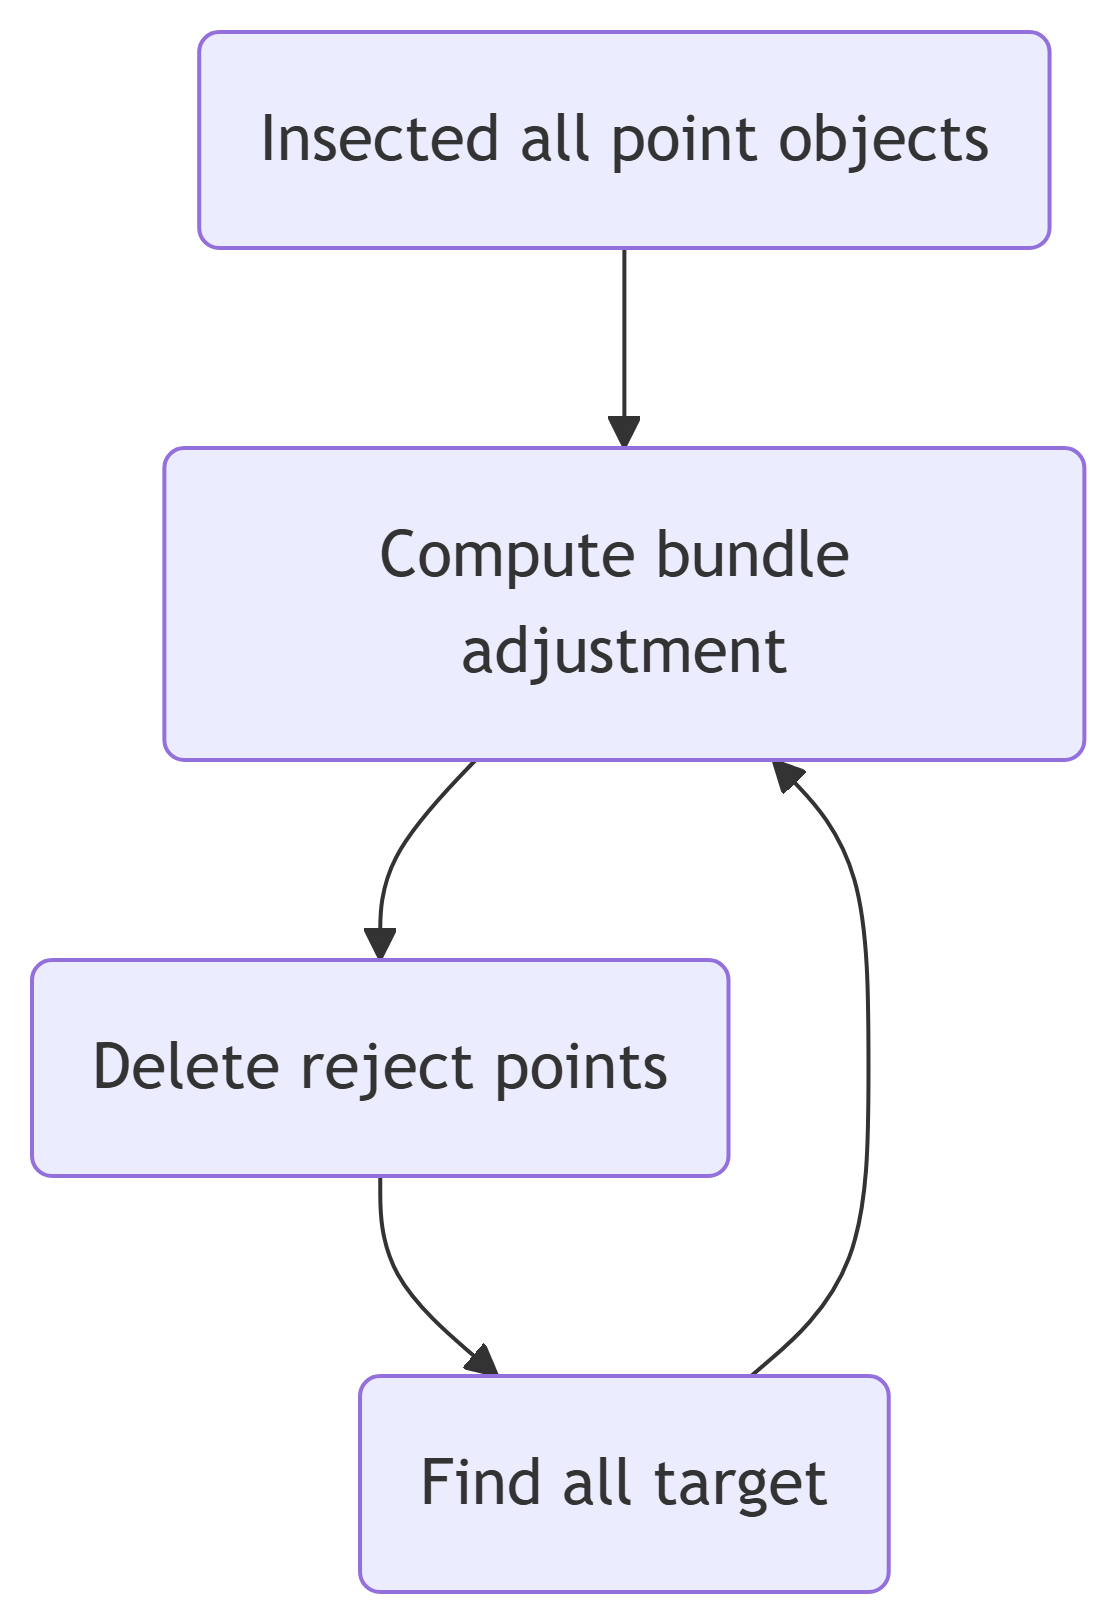
\includegraphics[width=2.91in,height=4.23in]{seagis-cal_files/figure-latex/mermaid-figure-2.png}

\emph{Adjustment: Compute bundle ajustment} \textgreater{} \emph{Delete
reject points} \textgreater{} \emph{Find target} \textgreater{}
\emph{Compute bundle ajustment\textgreater{} Delete reject points}
\textgreater{} \emph{Compute bundle ajustment} (Final)
\emph{\textgreater{}}

\chapter{Manual CAL (pt/br)}\label{manual-cal-ptbr-1}

\section{\texorpdfstring{\emph{Quick
Guide}}{Quick Guide}}\label{quick-guide-1}

\begin{quote}
Guia Rápido
\end{quote}

Utilize este guia para percorrer, passo a passo, o processo de
calibração de um sistema de câmeras estéreo. Após capturar e transferir
as imagens de um cubo de calibração, siga as etapas descritas a seguir.

Este guia pressupõe que você já possui arquivos de câmera
(\textbf{.CamCAL}) para iniciar a calibração. Caso isso não seja
verdade, consulte a página de download do software
(\href{https://www.seagis.com.au/download.php}{aqui}) para encontrar
arquivos de câmera comumente utilizados, entre em contato conosco para
obter assistência ou consulte a seção Section~\ref{sec-cameras} para
criar os arquivos necessários.

\begin{tcolorbox}[enhanced jigsaw, opacityback=0, colback=white, colframe=quarto-callout-caution-color-frame, left=2mm, leftrule=.75mm, toprule=.15mm, rightrule=.15mm, breakable, arc=.35mm, bottomrule=.15mm]
\begin{minipage}[t]{5.5mm}
\textcolor{quarto-callout-caution-color}{\faFire}
\end{minipage}%
\begin{minipage}[t]{\textwidth - 5.5mm}

É importante iniciar com arquivos de câmera que você saiba que estão
corretos.

\end{minipage}%
\end{tcolorbox}

\subsection{\texorpdfstring{\emph{Organize the
data}}{Organize the data}}\label{organize-the-data-1}

\begin{quote}
\emph{Organize os dados}
\end{quote}

\begin{enumerate}
\def\labelenumi{\arabic{enumi}.}
\item
  Usando o \textbf{Explorador de Arquivos do Windows}, crie um novo
  diretório (pasta) para o projeto.
\item
  Copie todos os arquivos de imagem associados à calibração para o novo
  diretório (nova pasta). Normalmente, serão dois arquivos de vídeo: um
  da câmera esquerda e outro da câmera direita.
\item
  Copie para esse diretório o arquivo de pontos do objeto
  (\textbf{.PtsCAL}) do cubo de calibração. \ul{Esse arquivo deve ser
  sempre uma cópia limpa do arquivo original.}
\item
  Copie para esse diretório os arquivos da câmera esquerda e direita
  (\textbf{.CamCAL}). Esses arquivos geralmente são provenientes da
  calibração anterior mais recente.
\end{enumerate}

\subsection{\texorpdfstring{\emph{Create a new
project}}{Create a new project}}\label{create-a-new-project-1}

\begin{quote}
\emph{Crie um novo projeto}
\end{quote}

\begin{enumerate}
\def\labelenumi{\arabic{enumi}.}
\item
  No CAL, crie um novo projeto usando \textbf{\emph{Project \textbar{}
  New project}}. Se necessário, você será solicitado a salvar quaisquer
  dados não salvos associados ao projeto atual. Insira um nome para o
  arquivo do projeto (por exemplo,
  \textbf{``\textbf{\emph{Calibration}}''}) e salve o arquivo do projeto
  no novo diretório que você acabou de criar para este projeto.
\item
  A criação de um novo projeto inicia um processo de assistente
  (\emph{wizard process}) que solicita a configuração do restante do
  projeto. Basta seguir as instruções, lembrando que todos os arquivos
  estão localizados no mesmo diretório, e que o CAL usará, por padrão, o
  diretório onde o novo arquivo de projeto foi criado.
\item
  Carregue os arquivos da câmera esquerda e direita (\textbf{.CamCAL}),
  conforme solicitado.
\item
  Carregue o arquivo do cubo de calibração (\textbf{.PtsCAL}), conforme
  solicitado.
\item
  Defina o diretório de imagens conforme solicitado. O diretório de
  imagens é automaticamente definido como o mesmo diretório do arquivo
  do projeto; portanto, se todos os arquivos da calibração estiverem em
  um único diretório, basta verificar e clicar em \textbf{OK}.
\item
  Salve o novo arquivo de medições conforme solicitado. Será necessário
  atribuir um nome a esse arquivo (por exemplo,
  \textbf{``\textbf{\emph{Measurements}}''}), e ele será o local onde as
  medições da calibração serão armazenadas.
\item
  Carregue a imagem da câmera esquerda. Normalmente, esse será o arquivo
  de vídeo da câmera esquerda, e ele será automaticamente adicionado à
  configuração da sequência de filmes (Movie sequence) da câmera
  esquerda. Caso existam mais arquivos de vídeo na sequência, eles podem
  ser adicionados nesse momento (ver \textbf{Sequências de filmes}). Em
  seguida, clique em \textbf{OK}.
\item
  Carregue a imagem da câmera direita. Normalmente, esse será o arquivo
  de vídeo da câmera direita, e ele será automaticamente adicionado à
  configuração da sequência de filmes da câmera direita. Caso existam
  mais arquivos de vídeo na sequência, eles podem ser adicionados nesse
  momento (ver \textbf{Sequências de filmes}). Em seguida, clique em
  \textbf{OK}.
\item
  A janela \textbf{\emph{Current project files}} (\emph{Arquivos do
  projeto atual}) será exibida. Todos os campos devem estar preenchidos,
  e todos os itens listados devem estar no mesmo diretório. Clique em
  \textbf{\emph{Close dialog}} (\emph{Fechar diálogo}).
\end{enumerate}

\begin{tcolorbox}[enhanced jigsaw, colframe=quarto-callout-note-color-frame, toprule=.15mm, opacitybacktitle=0.6, opacityback=0, bottomtitle=1mm, colback=white, coltitle=black, left=2mm, toptitle=1mm, titlerule=0mm, leftrule=.75mm, title=\textcolor{quarto-callout-note-color}{\faInfo}\hspace{0.5em}{Note}, rightrule=.15mm, arc=.35mm, breakable, bottomrule=.15mm, colbacktitle=quarto-callout-note-color!10!white]

Se houver dificuldades para chegar a esse ponto, consulte
\textbf{\emph{Creating new projects and data organization}}(), que
fornece mais detalhes ou mostra como configurar o projeto manualmente.

\end{tcolorbox}

\subsection{Medições}\label{mediuxe7uxf5es-2}

\subsection{Ajuste}\label{ajuste-2}

\begin{enumerate}
\def\labelenumi{\arabic{enumi}.}
\item
  Após concluir todas as medições de imagem, calcule o ajuste de feixe
  usando Ajuste \textbar{} Calcular ajuste de feixe.
\item
  Se você receber uma mensagem de aviso sobre medições de distância
  excluídas ou baixa precisão relativa, ignore-a por enquanto. Se o
  ajuste falhar, consulte os motivos pelos quais um ajuste de feixe pode
  falhar. Se ainda estiver com dificuldades para obter resultados que
  não convergem, tente uma solução apenas com a face frontal, descrita
  em Ajustes com falha em um cubo de calibração SeaGIS.
\item
  Quando o ajuste for bem-sucedido, siga os passos abaixo para produzir
  um conjunto ``limpo'' de medições de imagem, sem rejeições:

  \begin{enumerate}
  \def\labelenumii{\arabic{enumii}.}
  \item
    i. Aceite os resultados do ajuste (usando o botão Aceitar
    resultados).
  \item
    ii. Exclua as medições rejeitadas usando Medição \textbar{} Excluir
    medições de ponto rejeitadas.
  \item
    iii. Procure por alvos ausentes usando Medição \textbar{} Encontrar
    alvos em todas as imagens.
  \item
    iv. Calcule outro ajuste de feixe (Ajuste \textbar{} Calcular ajuste
    de feixe) e aceite os resultados.
  \item
    v. Exclua as medições rejeitadas usando Medição \textbar{} Excluir
    medições de ponto rejeitadas.
  \item
    vi. Calcule um ajuste de feixe final (Ajuste \textbar{} Calcular
    ajuste de feixe). Neste ponto, você deverá ter um ajuste de feixe
    correto. Verifique o seguinte no resumo de Ajuste (uma mensagem de
    aviso alertará sobre possíveis problemas de medição de distância e
    precisão relativa). Você deverá ter \textbf{zero} \emph{Eligible
    image measurements} excluídas e \textbf{zero} \emph{Eligible
    distance measurements} excluídas. Medições de distância excluídas
    podem ser causadas por um cubo montado incorretamente, cubo
    danificado ou medição de locais de pontos de ressecção incorretos --
    este problema deve ser corrigido. Verifique se o valor de precisão
    relativa está de acordo com o esperado para o seu sistema de câmera
    e método de calibração. O CAL possui alguns avisos integrados com
    base em cenários típicos de calibração: geralmente melhor que
    \textbf{1:10.000} para uma calibração estéreo de um sistema de
    câmera de alta definição usando o hardware de calibração SeaGIS.
    Valores mais baixos podem ser causados \hspace{0pt}\hspace{0pt}por
    baixa visibilidade, imagens desfocadas, iluminação inadequada (baixo
    contraste do alvo), número insuficiente de pontos medidos ou cubo
    muito distante das câmeras. Clique em Aceitar resultados.
  \end{enumerate}
\end{enumerate}

\textbf{Observe que o ajuste do feixe precisa ter qualidade aceitável
antes de prosseguir.}

\subsection{Geração de arquivos de câmera
estéreo}\label{gerauxe7uxe3o-de-arquivos-de-cuxe2mera-estuxe9reo-1}

Note, todas as operações de menu mencionadas nesta seção estão em
\emph{Measurement} \textbar{} \emph{Stereo constraints}.

\begin{enumerate}
\def\labelenumi{\arabic{enumi}.}
\item
  Configure as restrições estéreo usando \emph{Configure stereo
  constraints} . Nesta caixa de diálogo, geralmente basta garantir que a
  câmera esquerda e a câmera direita estejam selecionadas corretamente
  e, em seguida, clicar no botão *Automatic* para gerar os pares
  esquerda/direita. Você receberá uma mensagem de erro se houver um
  número diferente de imagens esquerda e direita medidas, pois o
  software não consegue criar pares estéreo -- você precisará encontrar
  e corrigir a imagem esquerda/direita que não possui uma imagem
  direita/esquerda correspondente (consulte Configurando restrições).
\item
  Estime as restrições usando *Estimating constraints* (consulte
  Estimando restrições). Um aviso será exibido se mais de quatro pares
  estéreo forem excluídos (consulte os comentários na próxima etapa).
\item
  Verifique a orientação relativa usando \emph{View stereo constraints}.
  Verifique se os resíduos de restrição são aceitáveis
  \hspace{0pt}\hspace{0pt}e se não houve muitas restrições que foram
  excluídas do cálculo (coluna \emph{Exclusions}). \textbf{Se mais de
  quatro restrições forem rejeitadas, verifique novamente a
  sincronização estéreo.} Para mais detalhes, consulte Visualizando as
  restrições.
\item
  Gere os arquivos da câmera estéreo usando Exportar arquivos da câmera
  estéreo (consulte Exportando arquivos da câmera estéreo).
\end{enumerate}

\subsection{Salvando resultados}\label{salvando-resultados-1}

A maneira mais simples de salvar o projeto e todos os dados associados é
fechar o CAL. O programa solicitará que você salve todos os dados não
salvos.

\subsection{Carregando calibrações
anteriores}\label{carregando-calibrauxe7uxf5es-anteriores-1}

Calibrações anteriores podem ser carregadas clicando duas vezes em um
arquivo de projeto CAL (.PrjCAL) no Explorador de Arquivos do Windows ou
usando o menu CAL \textgreater{} Projeto \textbar{} Ler do arquivo.

Se arquivos (como arquivos de câmera, arquivo de pontos do objeto ou
arquivo de medição) originalmente associados ao projeto tiverem sido
movidos para uma unidade e/ou pasta diferente, o projeto será corrompido
e você precisará recriá-lo manualmente, localizando e carregando os
arquivos necessários. Consulte Recriando um projeto de calibração a
partir de dados existentes.

\section{\texorpdfstring{\emph{General}}{General}}\label{general-1}

\section{\texorpdfstring{\emph{Installation
details}}{Installation details}}\label{installation-details-1}

\section{\texorpdfstring{\emph{Project
files}}{Project files}}\label{project-files-1}

Reading and writing to file

\section{\texorpdfstring{\emph{Cameras}}{Cameras}}\label{cameras}

\begin{quote}
\emph{Câmeras}
\end{quote}

O acesso às informações da câmera e às operações específicas da câmera é
feito por meio do menu \textbf{\emph{Camera}}.

As informações da câmera são armazenadas em um arquivo (um arquivo
separado para cada câmera). Os nomes dos arquivos de câmera atuais são
armazenados no arquivo do projeto e são carregados automaticamente
quando o CAL é iniciado. Observe que esses arquivos de câmera possuem a
extensão \textbf{.CamCAL}. Esses arquivos são diferentes dos arquivos de
câmera estéreo (com extensão \textbf{.Cam}), que o CAL exporta para uso
em softwares de medição estéreo, como o \textbf{EventMeasure} ou o
\textbf{StereoLib}.

\subsection{\texorpdfstring{\emph{Reading and writing to
file}}{Reading and writing to file}}\label{reading-and-writing-to-file-1}

\begin{quote}
\emph{Leitura e gravação em arquivo}
\end{quote}

As informações da câmera podem ser gravadas em um arquivo ou lidas a
partir de um arquivo. Para ler ou gravar um arquivo de câmera, utilize o
comando de menu \textbf{\emph{Camera \textbar{} Left \textbar{} Read
from file}} ou \textbf{\emph{Camera \textbar{} Left \textbar{} Write to
file}}. Comandos idênticos estão disponíveis para a câmera direita.

Se uma nova câmera for lida a partir de um arquivo ou salva em um
arquivo com um nome diferente, essa alteração será atualizada no arquivo
de projeto atual.

\subsection{\texorpdfstring{\emph{Editing camera
parameters}}{Editing camera parameters}}\label{editing-camera-parameters}

\begin{quote}
\emph{Edição de parâmetros da câmera}
\end{quote}

Para visualizar ou editar os parâmetros de uma câmera, utilize o comando
de menu \textbf{Camera \textbar{} Left \textbar{} Edit parameters} (ou
\textbf{Camera \textbar{} Right \textbar{} Edit parameters} para a
câmera direita). Será exibida uma janela com os seguintes itens:

\begin{longtable}[]{@{}ll@{}}
\toprule\noalign{}
\endhead
\bottomrule\noalign{}
\endlastfoot
& \\
& \\
& \\
& \\
& \\
& \\
& \\
& \\
& \\
& \\
& \\
& \\
& \\
& \\
& \\
\end{longtable}

Itens com um visto verde ao lado podem ser editados dando um duplo
clique no item e digitando um novo valor. Os itens na coluna
\textbf{Units} indicam as unidades do parâmetro. Os valores na coluna
\textbf{Precision} podem ser \textbf{``Fixed parameter''} (parâmetro
fixo) ou um valor numérico. A ausência de valor indica que o parâmetro
da câmera ainda não foi estimado por um ajuste de feixe; já um valor
numérico indica que o parâmetro foi estimado pelo ajuste de feixe, e
esse valor corresponde à precisão do parâmetro.

Os parâmetros \textbf{X Pixel size} e \textbf{Y Pixel size} são
propriedades da câmera e, em geral, podem ser encontrados no site do
fabricante ou em uma ficha técnica ou folha de especificações da câmera.
Frequentemente, o tamanho do pixel precisa ser derivado a partir do
tamanho do sensor da câmera e do formato da imagem. Normalmente, o
fabricante informa esses valores em unidades de micrômetros.
Certifique-se de converter os valores para milímetros (mm) ao inseri-los
como parâmetros da câmera.

Para calibrações de câmera subaquáticas utilizando uma porta plana do
invólucro da câmera, o valor da distância focal em água será
aproximadamente \textbf{4/3} do valor no ar (por exemplo, uma lente com
distância focal de 4,8 mm no ar terá aproximadamente 6,4 mm na água).
Certifique-se de considerar o efeito de quaisquer adaptadores de lente
grande-angular.

Quando uma nova câmera estiver sendo calibrada (isto é, não existe um
arquivo \textbf{.CamCAL} prévio), será necessário especificar:
\textbf{Image rows}, \textbf{Image columns}, \textbf{X Pixel size},
\textbf{Y Pixel size}, e estimar a \textbf{Focal length}. Todos os
demais parâmetros da câmera podem ser inicialmente estimados como zero,
tendo seus valores determinados durante o processo de calibração.

\subsection{\texorpdfstring{\emph{Fixing camera
parameters}}{Fixing camera parameters}}\label{fixing-camera-parameters-1}

\section{\texorpdfstring{\emph{Pictures}}{Pictures}}\label{pictures-1}

\section{\texorpdfstring{\emph{Images and
orientations}}{Images and orientations}}\label{images-and-orientations-1}

\section{\texorpdfstring{\emph{Object points and
distances}}{Object points and distances}}\label{object-points-and-distances-1}

\section{\texorpdfstring{\emph{Measurement}}{Measurement}}\label{measurement}

\begin{quote}
\emph{Medições}
\end{quote}

Esta seção aborda o processo de realização de medições de pontos, bem
como descreve o uso dos itens do menu \emph{Measurement}.

\subsection{Pontos de Medida}\label{pontos-de-medida}

\emph{Point measurement}

\subsection{Salvando e lendo as
medidas}\label{salvando-e-lendo-as-medidas-1}

\emph{Saving and reading measurements}

\subsection{Convertendo vídeos para
JPEG}\label{convertendo-vuxeddeos-para-jpeg-1}

\begin{quote}
\emph{Convert movie to JPEG}
\end{quote}

\subsection{Frames deslocados}\label{frames-deslocados-1}

\emph{Offset frames}

\subsection{Visualizar dados de
orientação}\label{visualizar-dados-de-orientauxe7uxe3o-1}

\emph{View orientation data}

\subsection{Visualizar/ Excluir medições de
imagem}\label{visualizar-excluir-mediuxe7uxf5es-de-imagem-1}

\emph{View/ delete image measurement}

\subsection{Resumo das medições de
imagem}\label{resumo-das-mediuxe7uxf5es-de-imagem-1}

\emph{Image measurement summary}

\subsection{Excluir medições da face
posterior}\label{excluir-mediuxe7uxf5es-da-face-posterior-1}

\begin{quote}
\emph{Delete back face measurement}
\end{quote}

Ao utilizar um cubo de calibração padrão da SeaGIS, é possível usar
\textbf{\emph{Measurement}} \textbf{\textbar{} \emph{Delete back face
measurement}} para remover todas as medições de imagem associadas a
pontos na face posterior do cubo. Essa função é uma ferramenta útil para
lidar com ajustes de feixe (bundle adjustments) que não convergem; ver
Section~\ref{sec-falha-ajustes}.

\subsection{Cálculo do centróide}\label{cuxe1lculo-do-centruxf3ide-1}

\emph{Centroiding}

\subsection{Restrições
Estereoscópicas}\label{restriuxe7uxf5es-estereoscuxf3picas-1}

\emph{Stereo constraints}

Esta seção aborda as opções de menu disponíveis em \emph{Measurement
\textbar{} Stereo constraints}. Essas operações são utilizadas para
configurar restrições estereoscópicas e calcular a \textbf{orientação
relativa} de um par de câmeras estereoscópicas (a orientação relativa
descreve a posição e a orientação de uma câmera em relação à outra e é
necessária para realizar medições com um sistema de câmeras
estereoscópicas). Essas opções são fornecidas principalmente para gerar
arquivos de câmera estereoscópica (extensão \textbf{.cam}) para uso com
\emph{PhotoMeasure}, \emph{EventMeasure} e \emph{StereoLib}.

Em calibrações de câmeras estereoscópicas, a câmera 1 refere-se à câmera
esquerda e a câmera 2 refere-se à câmera direita. O CAL mantém um
sistema de numeração, em vez de utilizar os termos ``Esquerda'' e
``Direita'', para facilitar calibrações genéricas em sistemas com mais
de duas câmeras.

\subsubsection{\texorpdfstring{\textbf{Configuração das
restrições}}{Configuração das restrições}}\label{configurauxe7uxe3o-das-restriuxe7uxf5es-1}

\emph{Configure constraints}

Use o comando de menu \emph{Configure stereo constraints} para definir
as restrições. Uma janela será exibida. O principal objetivo dessa
janela é permitir a definição de pares estereoscópicos de imagens
esquerda e direita, a partir dos quais a orientação relativa das câmeras
pode ser determinada.

Selecione a câmera esquerda (\emph{Left camera}) e a câmera direita
(\emph{Right camera}) apropriadas usando as caixas de seleção. Na
maioria dos casos, o restante da configuração pode ser realizado
utilizando o botão \emph{Automatic}. Ao clicar em \emph{Automatic}, a
lista de pareamentos será preenchida com combinações de nome do arquivo
da esquerda (nº do frame, nº da câmera) e nome do arquivo da direita (nº
do frame, nº da câmera). Verifique se os pareamentos representam pares
estereoscópicos válidos; caso contrário, será necessário editar a lista
manualmente. Observe que, em calibrações estereoscópicas padrão, a
câmera 1 corresponde à câmera esquerda e a câmera 2 à câmera direita.

Para excluir um pareamento, selecione-o e clique no botão \emph{Delete}.
Para adicionar um pareamento manualmente, selecione um \textbf{Filename}
da câmera esquerda (nº do frame, nº da câmera) e um \textbf{Filename} da
câmera direita (nº do frame, nº da câmera) e clique em \textbf{Add}. Se
algum dos dados recém-adicionados já estiver presente na lista atual de
pareamentos, ele será automaticamente removido e substituído pelo novo
pareamento estereoscópico.

Clique em \textbf{OK} para aceitar a nova configuração ou em
\textbf{Cancel} para ignorar as alterações.

\subsubsection{\texorpdfstring{\textbf{Estimar
restrições}}{Estimar restrições}}\label{estimar-restriuxe7uxf5es}

\emph{Estimate constraints}

Depois que as restrições estiverem configuradas, a \textbf{orientação
relativa} pode ser estimada. Utilize o comando de menu \emph{Estimate
constraints}. Uma janela será exibida mostrando a orientação relativa
calculada. Os detalhes dessa janela são explicados na seção
\textbf{Viewing the relative orientation}.

Se \textbf{mais de quatro} pares estereoscópicos apresentarem exclusões
associadas, será exibida uma mensagem de aviso. A presença de mais de
quatro pares estereoscópicos com exclusões indica possíveis problemas de
\textbf{sincronização estereoscópica} ou, alternativamente, problemas no
\textbf{ajuste de feixe} (ver \textbf{\emph{Viewing the constraints}}
\{Section~\ref{sec-view.constraint}\} abaixo).

\subsubsection{\texorpdfstring{\textbf{Visualização das
restrições}}{Visualização das restrições}}\label{visualizauxe7uxe3o-das-restriuxe7uxf5es}

\textbf{\emph{Viewing the constraints}}

Depois que as restrições estereoscópicas forem configuradas (ver
\textbf{Configuring constraints}) e estimadas (ver \textbf{Estimating
constraints}, ou estimadas durante um ajuste de feixe), a qualidade da
estimativa pode ser avaliada usando o comando de menu \emph{View stereo
constraints}. Esse comando abre uma janela que exibe cada pareamento
estereoscópico em uma linha, iniciando com o \emph{Filename} da câmera
esquerda e da câmera direita (número do frame, número da câmera).

As colunas seguintes apresentam os \textbf{resíduos} para \emph{Base},
\emph{Delta omega}, \emph{Left phi}, \emph{Left kappa}, \emph{Right phi}
e \textbf{\emph{Right kappa}}. Os resíduos correspondem à diferença
entre a orientação relativa de cada par estereoscópico esquerda/direita
individual e a \textbf{orientação relativa média} calculada a partir de
todos os pares estereoscópicos.

A coluna final lista quaisquer componentes que tenham sido
automaticamente excluídos do cálculo da orientação relativa com base em
seus resíduos (ver \emph{Stereo constraints} para a definição dos
limiares dessas exclusões e para saber quando esses limiares podem
precisar ser ajustados). A magnitude dos resíduos das restrições
estereoscópicas depende, em grande parte, da qualidade da sincronização
das câmeras estereoscópicas. Se uma das restrições apresentar muitos
componentes excluídos, deve-se suspeitar que a sincronização
estereoscópica desse pareamento esquerda/direita esteja incorreta. Isso
frequentemente ocorre devido a movimento excessivo do sistema de câmeras
e/ou da estrutura de calibração, em combinação com um pequeno erro de
sincronização --- possivelmente inferior a um frame --- ou ainda devido
a um erro na seleção do par estereoscópico durante a configuração das
restrições (ver \textbf{Configuring constraints}).

Se muitos dos pares estereoscópicos estiverem sendo excluídos e a
sincronização e a configuração dos pares estiverem corretas, pode ser
necessário \textbf{aumentar os limiares de exclusão}. Para isso, aumente
os valores de \emph{Critical value for base rejection} e/ou
\emph{Critical value for orientation rejection} em \textbf{Stereo
constraints}, e então reestime as restrições conforme descrito em
\textbf{Estimating constraints}. Sempre investigue a sincronização das
imagens estereoscópicas e o pareamento das imagens como a principal
causa das rejeições antes de ajustar esses limiares.

\begin{tcolorbox}[enhanced jigsaw, colframe=quarto-callout-note-color-frame, toprule=.15mm, opacitybacktitle=0.6, opacityback=0, bottomtitle=1mm, colback=white, coltitle=black, left=2mm, toptitle=1mm, titlerule=0mm, leftrule=.75mm, title=\textcolor{quarto-callout-note-color}{\faInfo}\hspace{0.5em}{Note}, rightrule=.15mm, arc=.35mm, breakable, bottomrule=.15mm, colbacktitle=quarto-callout-note-color!10!white]

É impossível obter uma sincronização consistentemente perfeita em
sistemas de câmeras de vídeo estereoscópicas que dependem de
sincronização visual. Nesses sistemas, o erro de sincronização pode
chegar, no pior caso, a meio frame. Esse erro de sincronização, em
combinação com o movimento do sistema de câmeras e/ou da estrutura de
calibração, inevitavelmente resultará em exclusões nas restrições
estereoscópicas. Em função desse erro de sincronização, é aceitável que
até quatro pares estereoscópicos apresentem exclusões.

\end{tcolorbox}

\subsubsection{\texorpdfstring{\textbf{Visualização da orientação
relativa}}{Visualização da orientação relativa}}\label{visualizauxe7uxe3o-da-orientauxe7uxe3o-relativa}

\emph{View relative orientation}

Utilize o comando de menu \emph{View relative orientation} para
visualizar os parâmetros atuais da orientação relativa. Uma janela será
exibida. Nessa janela, a origem dos parâmetros(\emph{Parameter source})
será indicada como \emph{Bundle adjustment} se os parâmetros tiverem
sido estimados no ajuste de feixe (ver \textbf{\emph{Stereo
constraints}}); caso contrário, será exibido \emph{Camera positions and
orientations}, o que significa que a orientação relativa foi derivada
das posições e orientações atuais das câmeras. O número de restrições
será igual ao número de restrições configuradas em
\textbf{\emph{Configuring constraints}}.

A separação da base, \emph{Base separation} (X), representa a separação
física entre as câmeras. Em configurações estereoscópicas típicas,
\emph{Delta omega}, \emph{Left kappa} e \emph{Right kappa} tendem a ser
\textbf{próximos de zero}, enquanto \emph{Left phi} e \emph{Right phi}
representam o grau de convergência interna de cada câmera (embora esses
valores também fiquem próximos de zero se as câmeras não convergirem).
Cada parâmetro possui uma precisão associada ao seu cálculo.

\subsubsection{\texorpdfstring{\textbf{Exportando os arquivos de câmera
estereoscópica}}{Exportando os arquivos de câmera estereoscópica}}\label{exportando-os-arquivos-de-cuxe2mera-estereoscuxf3pica}

\emph{Exporting stereo camera files}

Para exportar arquivos de câmera estereoscópica, as restrições
estereoscópicas devem estar configuradas (ver \textbf{\emph{Configuring
constraints}}), estimadas (ver \textbf{\emph{Estimating constraints}},
ou estimadas durante um ajuste de feixe) e os resultados verificados
(ver \textbf{\emph{Viewing the constraints}}). Em seguida, os arquivos
de câmera estereoscópica podem ser criados usando o comando de menu
\emph{Export stereo camera files}.

Se as restrições não tiverem sido configuradas ou estimadas, será
exibida uma mensagem de erro. Inicialmente, os parâmetros da câmera
esquerda serão mostrados em uma janela. Clique no botão \emph{Close} da
caixa de diálogo e uma mensagem solicitará que você salve os parâmetros
da câmera esquerda. Clique em \emph{Yes}, e uma janela padrão do Windows
será exibida, permitindo selecionar o nome do arquivo de câmera
estereoscópica para a câmera esquerda.

Após o salvamento do arquivo da câmera esquerda, uma nova janela será
exibida com os parâmetros da câmera direita. Clique no botão
\textbf{Close} da caixa de diálogo, e uma mensagem solicitará que você
salve os parâmetros da câmera direita. Clique em \textbf{Yes} para abrir
a janela do Windows, na qual será possível selecionar o nome do arquivo
da câmera direita.

\subsection{Ressecção de todas as
imagens}\label{ressecuxe7uxe3o-de-todas-as-imagens-1}

O comando de menu Medição \textbar{} Ressecção de todas as imagens na
janela principal do CAL calcula uma ressecção em todas as imagens
associadas ao projeto atual. Ao término do processo de ressecção, uma
janela com um relatório resumido é exibida. A janela lista todas as
imagens envolvidas na operação de ressecção, se a ressecção foi
bem-sucedida e o erro RMS associado à ressecção. Consulte os botões
Ressecção e Encontrar alvos automaticamente para obter mais informações
sobre ressecções. Observe que pelo menos quatro pontos de ressecção
devem ser medidos em uma imagem antes que ela possa ser ressecada.

Essa opção geralmente não é usada, pois as imagens normalmente são
ressecadas individualmente à medida que são medidas.

\subsection{Encontrar alvos em todas as
imagens}\label{encontrar-alvos-em-todas-as-imagens-1}

O comando de menu Medição \textbar{} Encontrar alvos em todas as imagens
executa um processo automático no qual todas as imagens do projeto atual
são carregadas e uma tentativa é feita para medir quaisquer pontos de
objeto não medidos em cada imagem. Enquanto esse processo estiver em
execução, uma janela de progresso será exibida. O processo pode ser
cancelado a qualquer momento clicando no botão Cancelar na janela de
progresso.

Essa opção geralmente é usada após um ajuste de feixe bem-sucedido. Após
um ajuste de feixe, os parâmetros da câmera apresentam melhor qualidade
e é provável que mais pontos de objeto possam ser medidos
automaticamente. O procedimento geral consiste em excluir as medições
excluídas pelo ajuste de feixe e, em seguida, executar esse processo
para medir automaticamente quaisquer pontos de objeto não medidos. O
ajuste de feixe pode então ser recalculado (consulte mais detalhes em
Calculando o ajuste).

Observe que esse processo tentará encontrar (em cada imagem) apenas os
pontos de objeto que atualmente não possuem medição. Se um ponto já
estiver medido, a medição atual do ponto será mantida sem alterações.

\subsection{Intersecção de todos os
pontos}\label{intersecuxe7uxe3o-de-todos-os-pontos-1}

O comando de menu Medição \textbar{} Intersecção de todos os pontos
utiliza as posições e orientações atuais da câmera para todas as imagens
e intersecta todas as medições da imagem para calcular as coordenadas do
objeto. Essa funcionalidade é usada para estimar as coordenadas do
espaço do objeto para pontos recém-medidos.

Ao realizar ajustes de feixe com cubos de calibração, essa opção não é
utilizada.

\subsection{Excluir medições de pontos
rejeitadas}\label{excluir-mediuxe7uxf5es-de-pontos-rejeitadas-1}

O comando de menu Medição \textbar{} Excluir medições de pontos
rejeitadas excluirá todas as medições de pontos que foram marcadas como
rejeitadas (as medições de pontos podem ser rejeitadas por ressecções,
intersecções ou ajuste de feixe; consulte Cores de pontos, Valores para
rejeição de medição). Essa função é normalmente usada após um ajuste de
feixe para excluir todas as medições de pontos rejeitadas.

Quarto enables you to weave together content and executable code into a
finished document. To learn more about Quarto see
\url{https://quarto.org}.

\section{\texorpdfstring{\textbf{Ajuste}}{Ajuste}}\label{ajuste-3}

\begin{quote}
\emph{Adjustment}
\end{quote}

Esta seção trata dos comandos de menu disponíveis no menu
\textbf{\emph{Adjustment}}. Esses comandos são usados para configurar e
executar um ajuste do fardo das imagens (\emph{bundle adjustment}).
Antes de calcular um ajuste de fardo, é necessário realizar a
\textbf{resseção} de todas as imagens, ver
Section~\ref{sec-pontos-medida}, e medir a maioria dos alvos na maioria
das imagens (preferencialmente, todos os alvos visíveis em todas as
imagens).

\subsection{Critérios de
convergência}\label{crituxe9rios-de-converguxeancia-1}

\begin{quote}
\emph{Convergence criteria}
\end{quote}

Durante o ajuste do fardo, os parâmetros (coordenadas dos pontos do
objeto, posições e orientações da câmera e parâmetros de calibração da
câmera) convergem para um valor final. O grau de convergência pode ser
ajustado com precisão, se necessário. Consulte também
Section~\ref{sec-cal-ajuste}.

\subsubsection{\texorpdfstring{\emph{Object
points}}{Object points}}\label{object-points-1}

\begin{quote}
\emph{Pontos do objeto}
\end{quote}

Para ajustar os \emph{critérios de convergência} dos pontos do objeto,
use o comando de menu \textbf{\emph{Adjustment \textbar{} Object point
convergence criteria}}. Uma janela será exibida, permitindo o ajuste dos
critérios de convergência. Esse valor geralmente pode ser definido como
1/1000 das unidades do espaço do objeto, por exemplo, 1 mícron se as
unidades do espaço do objeto forem milímetros.\footnote{Portanto, 10
  mícrons se a unidade de espaço do objeto for em centímetros (1 cm =
  10000 mícrons).}

\subsubsection{\texorpdfstring{\emph{Camera positions and
orientations}}{Camera positions and orientations}}\label{camera-positions-and-orientations-1}

\begin{quote}
\emph{Posições e orientações da câmera}
\end{quote}

Para ajustar os \emph{critérios de convergência} da posição e orientação
da câmera, use o comando de menu \textbf{\emph{Adjustment \textbar{}
Camera position and orientation convergence criteria}}. Uma janela será
exibida, permitindo o ajuste dos critérios de convergência. Há dois
valores: um para as orientações da câmera em unidades de segundos de
arco e outro para a posição da câmera. As unidades para a posição da
câmera serão em unidades do espaço do objeto x 1000. Os valores padrão
são 1 segundo de arco para orientação e 1/1000 das unidades do espaço do
objeto para posição (por exemplo, 1 mícron se as unidades do espaço do
objeto forem milímetros).

\subsubsection{\texorpdfstring{\emph{Camera
parameters}}{Camera parameters}}\label{camera-parameters-1}

\begin{quote}
\emph{Parâmetros da câmera}
\end{quote}

Os \emph{critérios de convergência} para os parâmetros da câmera podem
ser definidos usando o comando de menu \textbf{\emph{Adjustment
\textbar{} Camera convergence criteria}}. Cada um dos parâmetros da
câmera (consulte Section~\ref{sec-editing-camera-parameters}) possui
\ul{seus próprios critérios de convergência}. A tabela a seguir fornece
os valores padrão para os critérios de convergência da câmera.

\subsection{Ajustes de
configuração}\label{ajustes-de-configurauxe7uxe3o-1}

\begin{quote}
\emph{Adjustment settings}
\end{quote}

\subsection{Cálculo do Ajuste}\label{cuxe1lculo-do-ajuste}

\begin{quote}
\emph{Computing the adjustment}
\end{quote}

Após todas as imagens serem ressecadas e os alvos medidos em todas elas,
o ajuste de feixe pode ser calculado. Para executar o ajuste de feixe,
use o comando de menu Ajuste \textbar{} Calcular ajuste de feixe na
janela principal do CAL. Uma janela de progresso é exibida com um botão
Cancelar. O ajuste pode ser cancelado a qualquer momento clicando no
botão Cancelar (o processo não será cancelado até que a iteração atual
seja calculada). A janela exibe informações sobre o progresso do ajuste
(o número da iteração) e o sigma zero (que indica a qualidade do ajuste
e idealmente deve estar próximo de 1). O ajuste primeiro calcula uma
solução inicial, seguida por uma série de soluções de reponderação, onde
as medições de baixa qualidade são removidas automaticamente do ajuste.
Finalmente, as precisões e correlações dos parâmetros são calculadas.

Nesta etapa, haverá um ajuste convergido com sucesso ou um ajuste que
não convergiu. Uma nova janela será exibida. Essa janela contém duas
caixas de listagem: a caixa de listagem superior exibe um resumo do
ajuste em texto, e a caixa de listagem inferior exibe detalhes sobre o
ajuste.

Uma caixa de mensagem pode ser exibida com avisos sobre medições de
distância excluídas e/ou baixa precisão relativa. Os avisos são baseados
em cenários típicos de calibração de câmeras estéreo usando o hardware
de calibração SeaGIS. Nesses casos, o ajuste final do feixe não deve
apresentar medições de distância excluídas, e há expectativas em relação
à precisão relativa. Veja detalhes nos tópicos a seguir. Ignore o aviso
se ele não se aplicar especificamente ao seu uso do CAL.

Considerando o resumo do ajuste, a primeira linha indicará se o ajuste
convergiu com sucesso ou se houve falha. Outras informações fornecidas
serão:

\begin{itemize}
\tightlist
\item
  Indica se as observações da imagem foram reponderadas para obter um
  sigma zero de 1 (consulte Precisão da medição da imagem) e se a
  reponderação foi bem-sucedida. O valor de sigma zero é fornecido,
  assim como a nova estimativa da precisão da medição da imagem.
\end{itemize}

\begin{itemize}
\tightlist
\item
  Indica se algum aspecto do processo de ajuste falhou e, em caso
  afirmativo, fornece uma indicação do que deu errado. Isso pode incluir
  falha na convergência dentro do número máximo de iterações (consulte
  Ajuste) ou falha na resolução das equações normais (isso geralmente
  indica que não foram medidos pontos de objeto suficientes em imagens
  suficientes ou pode ser causado por restrições de pontos de objeto sem
  sentido).
\end{itemize}

\begin{itemize}
\tightlist
\item
  O resíduo médio da imagem (\textbf{geralmente deve ser sempre menor
  que 0,3 pixels}).
\end{itemize}

\begin{itemize}
\tightlist
\item
  O número total de parâmetros do modelo de ajuste, parâmetros restritos
  e redundâncias. \textbf{O número de redundâncias para uma calibração
  de câmera estéreo geralmente será da ordem de 5.000}.
\end{itemize}

\begin{itemize}
\tightlist
\item
  O número de medições de imagem e distância elegíveis e excluídas, e
  restrições de pontos de objeto. As medições excluídas não atenderam
  aos parâmetros definidos em Valores para rejeição de medição. Após um
  ajuste inicial, pode haver muitas medições de imagem elegíveis
  excluídas. Isso é normal. Ao usar o hardware de calibração do SeaGIS
  (um cubo), não deve haver nenhuma medição de distância elegível
  excluída -- isso pode indicar: um cubo montado incorretamente, um cubo
  danificado ou localizações de pontos de ressecção medidas
  incorretamente.
\end{itemize}

\begin{itemize}
\tightlist
\item
  Avisos se houver pontos no espaço do objeto que não possuem
  coordenadas estimadas. Isso ocorrerá se novos pontos do objeto forem
  adicionados sem estimativas de coordenadas (isso nunca deve acontecer
  com projetos de cubo de calibração). Use a interseção para estimar as
  coordenadas (consulte Interseccionar todos os pontos).
\end{itemize}

\begin{itemize}
\tightlist
\item
  Avisos se houver distâncias medidas para pontos do objeto que não
  existem ou para pontos do objeto que não possuem coordenadas
  estimadas.
\end{itemize}

\begin{itemize}
\tightlist
\item
  Avisos se houver posições de câmera não selecionadas (consulte Medição
  de ponto).
\end{itemize}

\begin{itemize}
\tightlist
\item
  Avisos se houver medições de imagem feitas para pontos de objeto que
  não existem ou para pontos de objeto que não possuem uma coordenada
  estimada.
\end{itemize}

\begin{itemize}
\tightlist
\item
  Avisos se houver medições associadas a uma câmera que não faz parte de
  um projeto (pode ocorrer se uma câmera for excluída de um projeto
  existente, mas ainda houver medições associadas à câmera excluída).
\end{itemize}

\begin{itemize}
\tightlist
\item
  Avisos se forem usadas restrições estéreo e as restrições não tiverem
  sido estimadas ou envolverem posições de câmera inválidas ou não
  estimadas (consulte Restrições estéreo).
\end{itemize}

\begin{itemize}
\tightlist
\item
  A precisão relativa (consulte View object point summary). Para a
  calibração estéreo de um sistema de câmera de alta definição usando o
  hardware de calibração do SeaGIS (um cubo), \textbf{esse valor deve
  ser em torno de 1:10.000} ou melhor. A precisão relativa pode ser
  prejudicada por: baixa visibilidade, iluminação inadequada (baixo
  contraste do alvo), imagens desfocadas, número insuficiente de pontos
  medidos ou cubo muito distante das câmeras.
\end{itemize}

Se o ajuste não convergir, os parâmetros que não estão convergindo serão
relatados. A não convergência geralmente está associada a uma geometria
de rede inadequada ou a um número insuficiente de medições em imagens
suficientemente diferentes (isso nunca deve ocorrer com redes de
calibração que envolvem cubos de calibração, como no Apêndice A -
Orientações do cubo de calibração). Para forçar a convergência do
ajuste, os critérios de convergência para os parâmetros que estão
falhando podem ser ajustados para forçar a rede a convergir (consulte
Critérios de convergência) ou o número máximo de iterações para o ajuste
do feixe pode ser aumentado temporariamente (consulte Ajuste).

A caixa de listagem Detalhes fornece informações mais detalhadas sobre
os resultados do ajuste. Todos os itens listados podem ser visualizados
com mais detalhes clicando duas vezes sobre o item. As seguintes
informações são fornecidas:

\begin{itemize}
\tightlist
\item
  Parâmetros da câmera: Para cada câmera, um resumo dos parâmetros da
  câmera. Essas informações são as mesmas exibidas em Edição de
  parâmetros da câmera. Certifique-se de que a distância focal esteja
  correta. Todos os outros parâmetros devem ter uma magnitude pequena --
  parâmetros com grande magnitude indicam um problema.
\end{itemize}

\begin{itemize}
\tightlist
\item
  Resumo dos pontos do objeto. Essas informações são as mesmas exibidas
  em Visualização do resumo dos pontos do objeto. \textbf{Verifique se a
  precisão relativa está correta. O número de pontos não estimados deve
  ser 0. O intervalo entre os desvios padrão máximo e mínimo dos pontos
  deve ser pequeno.} Se o desvio padrão máximo dos pontos for muito
  grande, isso indica que alguns pontos do objeto não foram medidos o
  suficiente para estimar as coordenadas com precisão. Esses pontos
  devem ser identificados e mais medições de imagem devem ser feitas
  nesses pontos.
\end{itemize}

\begin{itemize}
\tightlist
\item
  Coordenadas/precisões dos pontos do objeto. Essas informações são as
  mesmas exibidas em Viewing and manipulating object space points
  (Visualização e manipulação de pontos no espaço do objeto).
  \textbf{Nesta janela, identifique os pontos que apresentam desvios
  padrão maiores que a média (sX, sY, sZ)}. Geralmente, eles terão um
  número menor de medições (Nº de Obs.) em comparação com outros pontos.
  É necessário realizar mais medições de imagem nesses pontos. Verifique
  rapidamente se as coordenadas dos pontos do objeto estão dentro do
  intervalo esperado.
\end{itemize}

\begin{itemize}
\tightlist
\item
  Orientação e posições da câmera (e observações da imagem). Essas
  informações são as mesmas exibidas em Dados de orientação da imagem.
  Nesta janela, examine todas as posições e orientações da câmera e
  certifique-se de que os valores sejam razoáveis
  \hspace{0pt}\hspace{0pt}(observe especialmente as posições da câmera
  que não se encaixam). \textbf{Observe a precisão das posições da
  câmera (sX, sY, sZ) e das orientações (sOmega, sPhi, sKappa), bem como
  o número de medições em cada imagem (Nº de obs.)}. Esses valores devem
  ter magnitude semelhante em todas as imagens. Se uma imagem apresentar
  um desempenho particularmente pior, pode ser porque ela não possui
  medições suficientes dos pontos do objeto ou porque a qualidade da
  imagem pode ser inferior. Você também pode examinar as medições e os
  resíduos de uma imagem específica clicando duas vezes nela, embora o
  Resumo de resíduos da imagem abaixo possa ser mais útil.
\end{itemize}

\begin{itemize}
\tightlist
\item
  Resumo de resíduos da imagem. Estas são as mesmas informações
  descritas em Resumo de medições da imagem. \textbf{Analise os resíduos
  médios da imagem e identifique quaisquer imagens que apresentem uma
  média visivelmente maior do que as demais.} Investigue as medições
  e/ou a qualidade da imagem associadas a essas imagens. Frequentemente,
  uma imagem com uma média alta pode ter pontos de ressecção mal
  identificados ou medições feitas em alvos mal identificados. Nesses
  casos, é prudente excluir todas as medições da imagem com uma média
  alta e medi-la novamente. Uma média alta também pode ser causada por
  baixa qualidade da imagem (geralmente desfoque de movimento).
\end{itemize}

\begin{itemize}
\tightlist
\item
  Todas as medições da imagem. Estas são as mesmas informações exibidas
  em Visualizar/excluir medições da imagem. Classifique os dados nesta
  janela clicando duas vezes na coluna Rejeitadas para trazer todas as
  medições rejeitadas para o topo. Observe se as medições rejeitadas
  tendem a estar associadas a um ou mais pontos do objeto. Nesse caso,
  investigue todas as medições até o(s) ponto(s) específico(s) do
  objeto, pois a medição pode ter sido feita no ponto errado.
\end{itemize}

\begin{itemize}
\tightlist
\item
  Medições de distância. Esta opção só será exibida se houver medições
  de distância. As informações são as mesmas exibidas em Visualizando e
  manipulando distâncias. Verifique se alguma distância está sendo
  excluída (isso não deve acontecer com um cubo de calibração e indica
  que o cubo ou os alvos nele contidos podem ter sido danificados
  fisicamente).
\end{itemize}

\begin{itemize}
\tightlist
\item
  Visualizar correlações. Clicar duas vezes neste item abre outra janela
  que permite visualizar as correlações entre os parâmetros. Insira o
  coeficiente de correlação desejado; quaisquer parâmetros acima do
  coeficiente de correlação especificado serão relatados. Você pode
  optar por incluir ou excluir os parâmetros de posição e orientação
  (orientação externa) da câmera, conforme necessário. Após a
  configuração, clique no botão Fechar caixa de diálogo e uma nova
  janela será exibida mostrando quaisquer parâmetros correlacionados. Se
  a janela estiver vazia, não havia parâmetros acima dos limites
  prescritos.
\end{itemize}

\begin{itemize}
\tightlist
\item
  Restrições estéreo e resíduos. Esses dados só aparecerão se você usar
  restrições estéreo no ajuste de feixe (consulte Restrições estéreo).
  As informações e a interpretação são as mesmas que em Visualizando as
  restrições. Se muitos dos componentes de restrição estéreo estiverem
  sendo excluídos, a ponderação da restrição pode precisar ser relaxada
  (consulte Restrições estéreo).
\end{itemize}

\begin{itemize}
\tightlist
\item
  ~Restrições estéreo -- orientação relativa. Esses dados só aparecerão
  se você usar restrições estéreo no ajuste de feixe (consulte
  Restrições estéreo). As informações e a interpretação são as mesmas
  que em Visualizando a orientação relativa.
\end{itemize}

Se o ajuste for bem-sucedido, o botão Aceitar na parte inferior da
janela será habilitado. Após avaliar os resultados do ajuste e
certificar-se de que o resultado é válido, clique no botão Aceitar para
adotar o resultado do ajuste de feixe. Ao clicar no botão Aceitar, os
parâmetros da câmera, as coordenadas dos pontos do objeto e as posições
e orientações da câmera são atualizados com os resultados calculados no
ajuste de feixe. Se o ajuste falhar ou o resultado não for satisfatório,
clique no botão Cancelar para ignorar os resultados do ajuste.
\textbf{Nunca aceite os resultados de um ajuste de feixe questionável}.

Após concluir um ajuste de feixe bem-sucedido, é recomendável excluir as
medições de imagem que foram excluídas pelo ajuste (consulte Excluir
medições de pontos rejeitadas).

Se houver muitos pontos do objeto que não foram medidos com sucesso
(como geralmente ocorre quando não há informações de calibração
anteriores para uma câmera), esses pontos agora devem ser medidos
automaticamente com sucesso. Assim que o ajuste de feixe for calculado
com sucesso, haverá parâmetros de calibração da câmera melhores,
permitindo que os alvos não medidos sejam medidos automaticamente. O
procedimento para medição automática de todas as imagens do projeto é
descrito em Encontrar alvos em todas as imagens. Após a medição de mais
alvos, o ajuste do feixe pode ser recalculado. Observe que nunca será
possível medir todos os alvos em todas as imagens, pois alguns alvos
inevitavelmente estarão ocluídos.

\subsection{Razões pelas quais um ajuste de feixe pode
falhar}\label{razuxf5es-pelas-quais-um-ajuste-de-feixe-pode-falhar-1}

Às vezes, o ajuste de feixe pode falhar, e pode ser difícil identificar
exatamente por que isso está acontecendo. A seguir estão algumas razões
e soluções comuns:

\begin{itemize}
\tightlist
\item
  O ajuste pode não convergir devido a uma ou duas medições realmente
  ruins. Se for possível forçar o ajuste a convergir ao menos uma vez,
  essas medições problemáticas serão identificadas e removidas.
\end{itemize}

\emph{Ajuste o máximo de interações usando o} Ajustment \textbar{}
Ajustment \emph{settings e ponha o} Maximum iterations \emph{em 500.}

\begin{itemize}
\tightlist
\item
  Medições insuficientes para pontos suficientes. Às vezes, há uma
  tendência de calcular o ajuste de feixe antes de realizar medições
  suficientes em um número adequado de pontos do objeto e em imagens
  suficientes. Quando isso ocorre, o ajuste de feixe pode falhar
  completamente ou não convergir. Nesse caso, é simplesmente necessário
  realizar mais medições. O ajuste de feixe depende de redundância
  (muitas medições) para detectar e eliminar de forma confiável medições
  errôneas. Se não houver medições suficientes, a detecção correta
  dessas medições incorretas torna-se difícil e pode levar à falha do
  ajuste de feixe.
\end{itemize}

\emph{Não se preocupe em calcular o ajuste de feixe até que toda a
sequência de calibração tenha sido medida (ver} Apêndice A ---
Orientações do cubo de calibração\emph{). Se o processo de centroiding
não estiver encontrando muitos pontos, tente ajustar o brilho e o
contraste da imagem para realçar os alvos} (Brightness and contrast).
\emph{Também pode ser necessário ajustar a configuração de centróide
``Minimum Pixel Intensity Range'', reduzindo esse valor (}Editing and
fine tuning settings\emph{).}

\begin{itemize}
\tightlist
\item
  Um ajuste pode falhar se pontos medidos tiverem sido atribuídos a um
  ID de ponto incorreto. Se um ponto for medido de forma consistente e
  receber um ID incorreto em muitas imagens, isso causará confusão no
  ajuste de feixe (ou seja, o ajuste de feixe não conseguirá identificar
  com precisão que o ponto incorreto foi medido). Isso pode se tornar um
  problema sério se os pontos iniciais de resseção forem identificados
  incorretamente, pois, nesse caso, todos os demais pontos do objeto
  medidos automaticamente na imagem provavelmente também serão
  identificados de forma incorreta.
\end{itemize}

\emph{Percorra todas as imagens e verifique cuidadosamente se os pontos
de resseção estão corretamente identificados em cada imagem. Se você
encontrar uma imagem com pontos de resseção medidos incorretamente, a
forma mais simples é excluir a imagem e medi-la novamente.}

\begin{itemize}
\tightlist
\item
  Se você estiver tendo dificuldades com um ajuste de feixe,
  especialmente se tiver aceitado os resultados de um ajuste ruim, é
  recomendável recarregar o arquivo original de pontos do objeto (uma
  versão ``limpa'' do arquivo, e não aquela criada pelo ajuste que está
  causando problemas; ver Reading the object point file).
\end{itemize}

\emph{Após recarregar uma versão ``limpa'' do arquivo de pontos do
objeto, utilize o comando de menu \textbf{Measurement \textbar{} Resect
all images} e, em seguida, calcule novamente o ajuste de feixe}.

\emph{Se isso não for bem-sucedido, recarregue uma versão limpa do
arquivo de pontos do objeto usando \textbf{Object points \textbar{} Read
from file}. Exclua todas as medições, exceto os pontos de resseção:
\textbf{Measurement \textbar{} View/delete image measurements}, ordene
pela coluna \textbf{Point ID} e apague todas as medições de pontos,
mantendo apenas os pontos de resseção (nos cubos SeaGIS, estes
correspondem aos pontos 100, 101, 102, 103 e 104).}

\emph{Em seguida, faça a resseção de todas as imagens com
\textbf{Measurement \textbar{} Resect all images}, depois localize os
alvos com \textbf{Measurement \textbar{} Find targets in all images} e,
por fim, recalcule o ajuste de feixe}

\begin{itemize}
\tightlist
\item
  Quando um ajuste não converge, examine o \textbf{relatório resumo dos
  resíduos de imagem} na janela \textbf{Adjustment results}. Observe os
  campos \textbf{Valid points} e \textbf{Average magnitude}.
\end{itemize}

\emph{Investigue qualquer imagem que apresente um \textbf{Average
magnitude} mais alto do que o habitual (qualquer valor superior a três
vezes a média) e qualquer imagem que tenha um número de \textbf{Valid
points} inferior ao esperado (menos da metade dos alvos medidos). Em
geral, a maneira mais simples é excluir essas imagens e medi-las
novamente.}

Veja também a seção a seguir.

\subsection{Falha de ajustes com um cubo de calibração
SeaGIS}\label{falha-de-ajustes-com-um-cubo-de-calibrauxe7uxe3o-seagis}

Frequentemente, a razão para a falha de um ajuste de feixe está
relacionada a \textbf{estimativas inadequadas dos parâmetros da câmera},
o que resulta em medições automáticas de imagem de baixa qualidade.
Quando se dispõem de boas estimativas dos parâmetros da câmera (obtidas
a partir de calibrações anteriores), geralmente não há problemas na
execução do ajuste. Quando o ajuste falha ao utilizar um \textbf{cubo de
calibração de duas faces}, uma estratégia útil é realizar a calibração
usando \textbf{apenas a face frontal do cubo}. Isso fornece boas
estimativas dos parâmetros da câmera, permitindo que, posteriormente,
seja calculada uma calibração utilizando ambas as faces do cubo.

Para chegar ao ponto em que o ajuste de feixe está falhando, presume-se
que você já tenha realizado um conjunto de medições no material de
calibração. As instruções abaixo assumem que um projeto já foi criado e
que existe um conjunto completo de medições:

\begin{itemize}
\item
  Salve uma cópia das medições realizadas até o momento usando
  \textbf{Measurement \textbar{} Write measurement file}. Nomeie o
  arquivo como \emph{``Complete''}, ou algo similar, para indicar que se
  trata do conjunto original completo de medições.
\item
  Carregue uma cópia original ``limpa'' do arquivo do cubo de calibração
  (.PtsCAL) usando \textbf{Object points \textbar{} Read from file}.
\item
  Exclua as medições referentes aos pontos da face traseira do cubo
  usando \textbf{Measurement \textbar{} Delete back face measurements}.
\item
  Realize a resseção de todas as imagens usando \textbf{Measurement
  \textbar{} Resect all images}.
\item
  Calcule o ajuste de feixe em \textbf{Adjustment \textbar{} Compute
  bundle adjustment}.
\item
  Supondo que o ajuste de feixe seja bem-sucedido, exclua as medições de
  pontos rejeitadas usando \textbf{Measurement \textbar{} Delete
  rejected point measurements}.
\item
  Reintroduza a face traseira do cubo utilizando \textbf{Measurement
  \textbar{} Find targets in all images}.
\item
  Execute um novo ajuste de feixe (agora utilizando os pontos medidos
  nas faces frontal e traseira do cubo) e prossiga da forma habitual
  após a conclusão bem-sucedida do ajuste de feixe.
\end{itemize}

\chapter{Apêndices}\label{apuxeandices-1}




\end{document}
